
\documentclass[12pt]{article} 
\usepackage{alphalph}
\usepackage[utf8]{inputenc}
\usepackage[russian,english]{babel}
\usepackage{titling}
\usepackage{amsmath}
\usepackage{graphicx}
\usepackage{enumitem}
\usepackage{amssymb}
\usepackage[super]{nth}
\usepackage{everysel}
\usepackage{ragged2e}
\usepackage{geometry}
\usepackage{fancyhdr}
\geometry{top=1.0in,bottom=1.0in,left=1.0in,right=1.0in}
\newcommand{\subtitle}[1]{%
  \posttitle{%
    \par\end{center}
    \begin{center}\large#1\end{center}
    \vskip0.5em}%

}
\usepackage{hyperref}
\hypersetup{
colorlinks=true,
linkcolor=blue,
filecolor=magenta,      
urlcolor=blue,
citecolor=blue,
}

\urlstyle{same}
\renewcommand*\familydefault{\ttdefault}
\EverySelectfont{%
\fontdimen2\font=0.4em% interword space
\fontdimen3\font=0.2em% interword stretch
\fontdimen4\font=0.1em% interword shrink
\fontdimen7\font=0.1em% extra space
\hyphenchar\font=`\-% to allow hyphenation
}

\pagestyle{fancy}
\lfoot[\vspace{-15pt} \hline]{\vspace{-15pt} \hline}
\rfoot[\vspace{-15pt} \hline]{\vspace{-15pt} \hline}
\cfoot[\thepage]{\thepage}
\lhead[\copyright 2020 $-$ \textit{All Rights Reserved} ]{\copyright 2020 $-$ \textit{All Rights Reserved}}
\rhead[Michael Brodskiy]{Michael Brodskiy}

\begin{document}

%------------------------------------------------------------------------------------------
% Title
%------------------------------------------------------------------------------------------

\author{Michael \textsc{Brodskiy}}
\title{Final Review Packet\\European History AP}
\subtitle{Mrs Fisher}
\date{April 28, 2020}
\maketitle
\begin{center}
    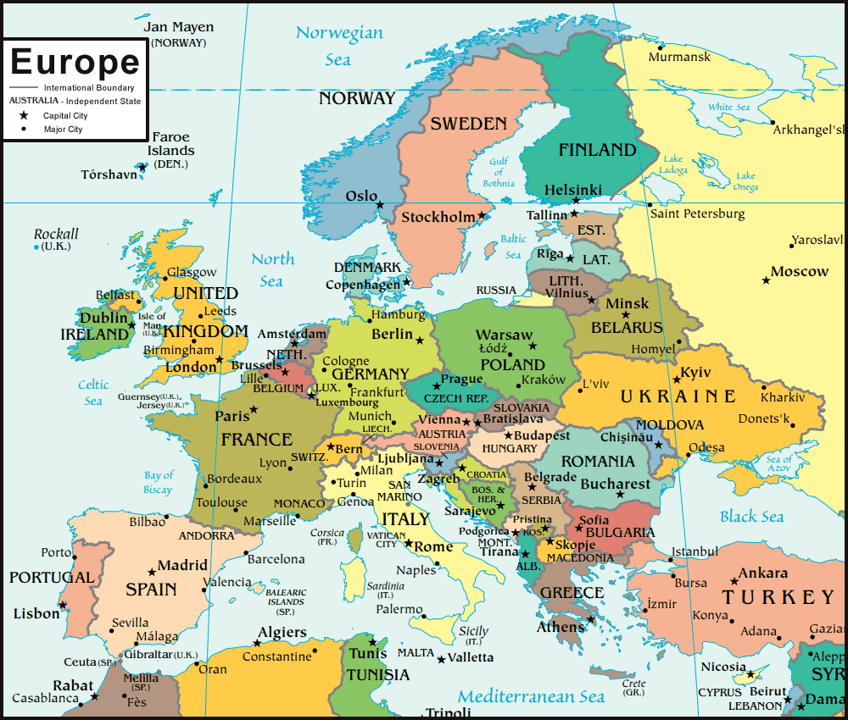
\includegraphics[width=\textwidth]{Images/Europa.png}
\end{center}
\newpage
\tableofcontents
\newpage

%------------------------------------------------------------------------------------------
% Questions
%------------------------------------------------------------------------------------------
\newpage
\begin{center}
\end{center}
\begin{center}
\end{center}
\begin{center}
\underline{\Huge The Renaissance}
\end{center}
\vspace{50pt}
\includegraphics[width=\textwidth]{Images/renaissance.png}
\newpage

\begin{center}
\section{\underline{Renaissance}}
\end{center}

\begin{enumerate}[label=]
\subsection{Causes}
\item
\end{enumerate}
\vspace{-35pt}
\begin{enumerate}

\item Philosophical/Religious $-$ During the Renaissance, the term \textit{secularism} came about. This refers to something that does not relate to religion, something down-to-earth. Many artists began to paint more secular pieces, which focused on individual traits, and many were based off of classical Greek and Roman works of art. Also, many philosophers revived classical Greek and Roman thinking, and, as such, more philosophes came about.

\item Political (city states) $-$ The Italian city states did not wage war against each other for quite a bit. This created an accumulation of wealth that permitted the cities to to begin the period known as the Renaisance.

\item Economic $-$ The Renaissance began because of accumulation of wealth in Italian city states. Many Italian cities were based off of merchants and trading, and this allowed great amounts of wealth to pour in.

\item Social $-$ People became a bit more down to earth because of the new Renaissance ideals, such as: Humanism, Individualism, and Secularism.

\subsection{Terms}

\item Humanism $-$ The call back to classical Greek and Roman antiquity. This included art, architecture, and philosophy.

\item Individualism $-$ The focus on the individual as opposed to god. This stressed the importance of self value and education.

\item Secularism $-$ Down-to-earth, or not relating to religious beliefs or a god.

\subsection{People}

\item Machiavelli $-$ The author of \textit{The Prince}. He wrote this book for Cesare Borgia to demonstrate what a true Prince should act like. One of the major questions in the book is: "Which is better, to be feared or to be loved." This book offers a perspective on the royal life during the Renaissance.

\item Christine de Pisan $-$ Pisan was best remembered for defending Women in \textit{The Book of the City of Ladies}. 

\item Valla $-$ Lorenzo Valla was an early example of a humanist. He believed that pleasing the human senses was of most importance. Also, he found that a document from the 700s that granted the church rights to lots of land was a forgery.

\item Petrarch $-$ Petrarch coined the term 'Renaissance.' He began the early humanist movement. 

\item Dante $-$ Dante is the author of \textit{The Divine Comedy}. This work is considered very, if not the most important work of the Middle Ages. 

\item Boccaccio $-$ Boccaccio was an important Renaissance humanist. He wrote his book, \textit{The Decameron} in a vernacular language (meaning everyday people could read it). \textit{The Decameron} takes place near the outskirts of Florence, Italy. There are twelve people who share stories with each other. These twelve people are spending time in the outskirts of Florence to escape the raging Black Death.

\item Medici Family $-$ The Medici Family was the wealthy merchant family of Florence during the Renaissance. Because they had the greatest wealth, they were essentially the ruling family. The wealth they poured into art and the city itself spurred what is known as the Renaissance.

\item Da Vinci $-$ Da Vinci is one of the most famous artists of the Renaissance era. He was a prolific producer of art, as well as an early researcher of science. He had drawings of human anatomy, flying contraptions, and other inventions.

\item Michelangelo $-$ Michelangelo is one of the most renowned Renaissance artists. He is most famous for his work on the Sistine Chapel. To paint the ceiling, he had to spend excruciating amounts of time on his back.

\item Raphael $-$ Raphael is another Renaissance era artist. His pieces emphasized individuality and human features, as opposed to the general style of the time.

\item Alexander VI $-$ He was a corrupt pope of the Borgia Family. He encouraged his son, named Cesare, to create an Italian state ruled by their family. Alexander believed that this state was to be created by any means necessary.

\item Julius II $-$ His nickname is the "Warrior-Pope." He was involved in a lot of wara and politics. In some cases, he personally led troops to war against his enemies. He is responsible for the creation of St. Peter's Basilica.

\item Leo X $-$ Leo is responsible for the selling of indulgences. He began to sell them to fund the building of St. Peter's Basilica. Later, he would be the Pope that condemns Luther for being a heretic.

\subsection{Northern Renaissance}

\item Erasmus $-$ Desiderius Erasmus is the most famous Northern Renaissance humanist. He was of Dutch origins. He wrote \textit{The Praise of Folly}, where wrote that people should study the Bible for themselves, and that Christianity at heart, not through ceremonies was the most important.

\item More $-$ More was an early example of a Utopian Socialist. He wrote a book titled \textit{Utopia}, which comes from roots meaning 'non-existent.' In his book, he states that the government is corrupt, and that private property should not exist. He was later executed by Henry VIII for not agreeing that Henry VIII was the head of the church.

\item Durer $-$ Albrecht Durer was a painter, mostly known for three works: \textit{Devil} (1513), \textit{Melancolia I} (1514), and \textit{Rhinoceros} (1515).

\item Printing Press $-$ The printing press was made in 1454. Its main creator was Johannes Gutenberg, known for the publication of \textit{The Gutenberg Bible}. The printing press would later spur the Reformation into action, as people began to read the Bible for themselves due to the possibility of mass production permitted by the printing press.

\subsection{Compare and Contrast the Italian and Northern Renaissances}

\item Similarities $-$ Both the Italian and Northern Renaissance were inspired by classical Greek and Roman antiquity, and, therefore, were both based off of the idea of humanism.

\item Differences $-$ As opposed to the North, Italian Renaissance artists focused more on secular works. The Northern States were inspired by Christianity, and, as a result of this, Northern humanists became known as Christian humanists.

\subsection{Effects}

\item Philosophical/Religious $-$ Due to the creation of the printing press, people would begin reading the bible for themselves. This would lead to the Reformation and other religious movements.

\item Political $-$ For the duration of the Renaissance, the Italian city-states would develop a policy known as Balance of Power. This meant that if one of the states got wealthier or more powerful, the other city-states would work to even it out. The militaries of the Italian city-states, however, would prove weak following an invasion of Italy which would result in the Habsburg-Valois Wars.

\item Economic $-$ Many powerful cities, in both Italy and the North. would arise. These cities would become major trade stops for other empires. One example of such would be Amsterdam, which, for a period of time, be the center of European trade.

\item Social $-$ Following the Renaissance, books such as Castiglione's \textit{Book of the Courtier}, and Machiavelli's \textit{The Prince} would put in place social guidelines on how people in certain positions should act.

\item Education $-$ As a result of the printing press, literacy rates rose. People began to become interested in writings, such as encyclopedias, and, of course, the Bible.

\newpage
\begin{center}
\end{center}
\begin{center}
\end{center}
\begin{center}
\underline{\Huge The New Monarchs}
\end{center}
\vspace{50pt}
\includegraphics[width=.9\textwidth]{Images/newmonarchs.jpg}
\newpage


\begin{center}
\section{\underline{The New Monarchs}}
\end{center}

\subsection{Causes}

\item Political $-$ The Renaissance had ushered in an era of relative peace. The New Monarchs saw this as a possibility to gain power, and, as such, they seized power.

\item Economic $-$ The New Monarchs were a direct result of the increased income during the Renaissance period. The New Monarchs needed greater revenue in order to crush political opponents and develop standing armies. As such, the period following the Renaissance was perfect for their rise.

\item Need for Permanent Standing Army $-$ The abundance of mercenaries during the Renaissance would allow for New Monarchs to establish permanent standing armies, which was something that had never been done by monarchs.

\item Taxation to Pay For Army and Bureaucracy $-$ Taxation resulted in even less money for the Peasants.

\item Classes
\begin{enumerate}[label=\arabic{*}.]
\setcounter{enumii}{36}
\item Nobles $-$ New Monarchs took power away from the nobility and placed it upon themselves. Such a move would result in a more centralized government, and thus, a more efficient bureaucracy.

\item Church $-$ As with the nobles, the New Monarchs reduced the power of the church. As such, the New Monarchs were able to create a more efficient and centralized government.

\item Middle $-$ In most of Europe, the middle class did not change very much during this time period. In Spain, however, the middle class would virtually disappear. Under the rule of Ferdinand and Isabella, the Reconquista began. This was a massive push to "Christianize" Spain. This would nearly wipe out the majority of the middle class, which consisted of the muslim Moors and Jewish people.

\end{enumerate}

\subsection{Political Situation $-$ 16\textsuperscript{th} Century}

\setcounter{enumi}{39}

\item Spain $-$ At the start of the 16\textsuperscript{th} century, Isabella had died. Ferdinand did find another queen, however they were not able to produce another heir, and, as such, Ferdinand did not have an heir from his new queen. Charles V was the most powerful ruler of Spain in the 16\textsuperscript{th} century. He fought the Habsburg-Valois war, sacked Rome in 1527, and established his main goal as the prevention of the spread of Protestantism.

\item France $-$ At the beginning of the 16\textsuperscript{th} century, France was ruled by Louis XII. He had a disastrous foreign policy, and, as such, he left an empire in trouble for his successor, Francis I. Francis I required for all bishops in churchs to be appointed by the King. He also implemented a direct tax on all property. 

\item England $-$ Before the beginning of the 16\textsuperscript{th} century, the War of the Roses was fought in England. The York family came out on top, and would then establish the Tudor dynasty. This would lead to the rise of Henry VII, the first Tudor king. Henry VII is best known for his establishment of the Star Chamber.  was the loyal right hand man of king Henry IV

\item Holy Roman Empire $-$ Maximilian I married Mary of Burgundy to obtain land in eastern France. This would spark the conflict between the House of Valois and the House of Habsburgs, and it would start the Habsburg-Valois War.

\subsection{Spain \& The Holy Roman Empire}

\item Ferdinand \& Isabella $-$ Ferdinand and Isabella ruled from 1479 to their respective deaths. Isabella died in 1504, and Ferdinand died in 1516. Together, they instigated the \textit{Reconquista}, or the reconquering of the Iberian Peninsula. They began the Catholic revival of Spain, driving out any non-Catholics. The Spanish Inquisition tortured non-Catholics into converting, fleeing Spain, or until death. This nearly destroyed the entire middle class of the Spanish Empire. 

\item Charles V $-$ Charles V was the most powerful ruler of Europe in the 16\textsuperscript{th} century. He inherited Spain and parts of most of the major contiguous European empires at the time. Leaders of the European countries were worried that Charles V would try to invade and create a world empire. 

\item Phillip II $-$ Phillip II is the son of Charles V. He is responsible for the unification of Spain with the Habsburgs. Phillip II married Mary, Queen of Scots. This showed a unification of Catholic leaders, and, as such, was a show of aggression to the English Protestants.

\subsection{England}

\item Henry VII $-$ Henry VII is the first King of the Tudor dynasty. He is best known for his establishment of the Star Chamber. His son is Henry VIII.

\item Henry VIII $-$ Henry VIII is the son of Henry VII. He married Catherine of Aragon to keep peace with Spain. Henry VIII is best known for having 6 wives. He wanted to divorce Catherine of Aragon because she only birthed daughters. The Pope, however, did not permit for Henry to divorce. As such, Henry VIII created the Anglican church through the acts of submission of clergy and supremacy. This established and declared the monarch of England the head of the Anglican church.

\item Elizabeth I $-$ Elizabeth was the daughter of Henry VIII and Anne Boleyn. She brang in an era of religious peace in England. She herself was protestant, and, as a result, she repealed any anti-protestant legislation. Her power was threatened when Mary, Queen of Scots came to England. Many people believed Mary was the true queen. Elizabeth kept Mary under house arrest, until it was revealed that there was a plan to assassinate Elizabeth. Mary was then beheaded.

\newpage
\begin{center}
\end{center}
\begin{center}
\end{center}
\begin{center}
\underline{\Huge The Age of Exploration}
\end{center}
\vspace{50pt}
\includegraphics[width=.9\textwidth]{Images/exploration.jpg}
\newpage

\begin{center}
\section{\underline{The Age of Exploration}}
\end{center}

\subsection{Causes}

\item Political $-$ People wanted to participate in exploration to become famous. This makes up the "Glory" component of the three G's.   

\item Economic $-$ Interest in trade and spice routes fueled countries to fund explorers. Also, tales of far lands made of gold and precious metals further increased interest in exploration. This makes up the "Gold" component of the three G's.

\item Technological $-$ New inventions, such as the rudder, a piece designed to facilitate the steering of a vessel, or the caravel, a smaller ship that was effective for travel, permitted countries to engage and fund exploration.

\item Religious $-$ Also, people wanted to spread their religion through exploration. This led to the creation of missionaries that would travel on ships. This makes up the "God" component of three G's.

\subsection{People}

\item Prince Henry the Navigator $-$ Prince Henry the Navigator was Portuguese. He supported the idea of exploration so greatly, that he himself sailed on exploration voyages. He began the Age of Exploration. 

\item Columbus $-$ Christopher Columbus reached the Bahamas and parts of North and South America, thinking that it was India. As such, he called the natives "Indians." Today it is questioned whether he was a great hero or an evil man due to his mistreatment of the Native Americans.

\item Magellan $-$ Ferdinand Magellan is famous for two things relating to exploration. First, he opened the Strait of Magellan, which was extremely useful for transportation between the east and west coasts of the Americas. Second, he was the first person to circumnavigate the world. 

\item Diaz $-$ Bartholomew Diaz is one of the most famous he explorers. He is best known for his rounding of the Cape of Good Hope in 1488.

\item Da Gama $-$ Vasco da Gama is most famous for discovering a water route to India. As a direct result, the whole Italian monopoly on Asian trade was destroyed.

\item Cortes $-$ Hernando Cortes is most famous for his conquering of the Aztecs. He was searching for a city of gold, and ended up claiming Mexico for the Spanish.

\item Pizzaro $-$ While Cortes conquered in the north, Francisco Pizzaro conquered the Incas in Peru. 

\subsection{Effect on the Americas}

\item Destruction of Civilizations $-$ A direct and almost immediate result of exploration was the destruction of indigenous peoples. Although the reasons for this varied, the two most important ones are conquest and disease. People such as Cortes and Pizzaro would conquer the natives they met. Disease wiped out more natives than any other factor, as the European diseases, such as smallpox, arrived. The natives did not have any tolerance to European diseases, and, as such, contracted the diseases easily. 

\item African Slavery $-$ The market for slaves began to grow greatly, as exploration into Africa became more prevalent. Developments such as the Triangle Trade made easy access to a lucrative business for merchants. As it is to this day, people will always need cheap labor, and, as a result, the slave market grew greatly.

\subsection{Effect on Europe}

\item Intellectual $-$ With the increasing sphere of European influence in explored regions following the unilateral growth of wealth the invested European powers, primarily Spain and Portugal, gained knowledge of world geography and sailing routes to the Americas and India with respect to the European mainland.

\item Economic $-$ The economy became increasing inundated with silver and gold which inadvertently created an increase in demand of these commodities further attributing to their affluent appeal. The routes by which exchanges of the aforementioned commodities took place enabled monopolies such as the British and Dutch East India Companies to extend their transnational operations.

\item Political $-$ The formation of monopolies would further attribute to the manifestation of capitalism with relatively smaller localized governments operating analogous to the monopolies and increasing their yields of production of profitable manufacture. This model spread through most of the explored regions and would accompany European colonialism within its sphere of influence.

\subsection{Colombian Exchange} 

\item Diseases $-$ During the Colombian Exchange, many diseases were brought to and from the Americas. Most notably, smallpox was brought to America, while syphilis was brought to Europe.

\item Food $-$ Many new crops were found. These crops facilitated subsistence farming and allowed for more food availability to the average European diet. Crops brought over include, but are not limited to corn, potatoes, tomatoes, and beans.

\begin{enumerate}[label=\arabic{*}.]
\setcounter{enumii}{67}
\item Potato on Population of Northern Europe $-$ The potato was one of the most robust crops brought to Europe. It could be grown in nearly any climate, and had a good amount of calories for sustenance. As such, the population began to grow due to the surplus of food now available.
\end{enumerate}
\setcounter{enumi}{68}
\item Price Revolution (Inflation) $-$ The Price Revolution was the sharp inflation which occurred during the late period of exploration. This began in Spain and spread to other European countries.

\begin{enumerate}[label=\arabic{*}.]
\setcounter{enumii}{69}
\item Causes $-$ One reason for the Price Revolution was the growing population. The abundance of new crops caused a decrease in infant mortality rates, and, as such, an increase in population. This population required more goods, which, especially in Spain due to the nearly nonexistent middle class, could not be provided. Another reason for this inflation was the influx of precious metals such as gold and silver.

\item Effects $-$ The Price Revolution caused the Spanish economy to collapse. Other countries were worried the same would happen to them, so exploration slowed down greatly.
\end{enumerate}

\newpage
\begin{center}
\end{center}
\begin{center}
\end{center}
\begin{center}
\underline{\Huge Religious Reformation}
\end{center}
\vspace{50pt}
\includegraphics[width=.9\textwidth]{Images/reformation.jpg}
\newpage

\setcounter{enumi}{71}
\section{\underline{Religious Reformation}}

\subsection{Causes}

\item Religious $-$ Sale of indulgences (essentially buying forgiveness for one's sins) and other "loose morals" angered people like Luther, who believed that religion was up to the people, not the priests. Also, Luther denounced pluralism and simony, as well as Absenteeism.

\item Political $-$ One movement that fueled the Reformation was Henry VIII's switch to Anglicanism. This separated England from the pope, and would result in further spread of Protestant ideals.

\item Economic $-$ The church would take part in simony, or the selling of church offices. Also, they would sell indulgences in order to fund exploits.

\item Social $-$ Many preachers who would read the Latin version of the bible would themselves be illiterate. As such, they would preach whatever would make them more successful.

\item Northern European Renaissance Humanism $-$ The most prominent North Renaissance Humanist, Desiderius Erasmus, inspired Martin Luther. In his book, \textit{The Praise of Folly}, he criticized the church for problems such as laernign about faith through clerics. He believed that people should read the Bible for themselves.

\item Reason's for Luther's Success $-$ Luther was successful because his ideas appealed to the masses. Many people believed in salvation by faith alone, and, as such, supported Luther and his criticism of the church.

\subsection{Effects}

\item Religious $-$ The Reformation resulted in the spread of major religions that branch from Catholicism, known as Protestantism (It comes from \textit{protesting} the Catholic faith).

\item Political $-$ The biggest political effect of the Reformation was the Thirty Years' War. The Protestant-Catholic split was exacerbated by the Catholic attempts of censorship of Protestant ideas. This would directly result in the Thirty Years' War, whichw as mainly fought in the region that, modern day, is Germany.

\item Economic $-$ The Reformation supported scientific thought and acceptance of new ideas. This would lead to new inventions, which made countries richer.

\item Social $-$ People became more interested in reading the Bible for themselves, and, as such, literacy rates increased quite a bit.

\subsection{Important People}

\item Wycliffe $-$ John Wycliffe was one of the earliest church reformers. He himself was a priest. He translated the Bible to English, and was eventually pronounced a heretic.

\item Huss $-$ Jan Huss was a Czech reformer. As with all religious reformers, he was declared a heretic and was excommunicated by the church. Later, he was executed by the Holy Roman Empire.

\item Luther $-$ Luther is the most well known supporter of the Reformation. He was a German peasant who became a Catholic monk. He always disliked the church system. The final straw was the sale of indulgences, which started his revolt against the Catholic church.

\item Zwingli $-$ Ulrich Zwingli was another reformer in Switzerland. Zwinglism was almost identical to Lutheranism, except for one point: they disagreed on the Lord's Supper, better known as communion. They met at the Marburg Colloquy to discuss combining their movements, however the idea of communion kept them apart. 

\item Calvin $-$ Calvin was another Protestant reformer. His focus on religion centered around the fact of predestination $-$ that it is predetermined, at birth, whether a person will go to heaven or hell. He created the Calvinist city that is now Geneva, Switzerland. Although it began as the second most popular sect of Protestantism, behind Lutheranism, it quickly became the definition of a reformed church.

\item Henry VIII $-$ Henry VIII formed the Anglican church, and, technically, was a religious reformer in England. He broke with the church in Rome, and made the monarch the leader of the Anglican church so that he could divorce.
    
\item Edward VI $-$ Edward VI is the son of Henry VIII. He had to take the throne at nine years old. He moved the church into an extremely Protestant direction.

\item Bloody Mary $-$ Better known as Mary Tudor, she is the daughter of Henry VIII. She is known as Bloody Mary because she burned many Protestants at the stake after she restored Roman Catholicism as the religion of England.

\item Elizabeth I $-$ Elizabeth I was the daughter of Henry VIII. She was a moderate ruler. Her policy was known as \textit{Politique}, where a monarch takes the middleground between religious extremes. She allowed sermons in English, allowed priests to marry, and made the Book of Common Prayer to unite churches.

\item Mary, Queen of Scots $-$ Also known as Mary Stuart, she fled to England, but was imprisoned by Elizabeth I. This was because many people believed Mary Stuart was the rightful queen. Mary was executed after an assassination attempt on Elizabeth I was unveiled.

\item Leo X $-$ Leo X was the first to sell indulgences. He intended this system to raise moeny to rebuild St. Peter's Basilica. He condemned Luther an outlaw, and excommunicated him from the church.

\item Tetzel $-$ Tetzel promoted the sales of indulgences. He was essentially the modern day equivalent of the marketing department. He is famous for the motto about indulgences that goes: "As soon as the coin in the coffer rings, the soul from purgatory springs."

\item Frederick, Duke of Saxony $-$ The Duke of Saxony protected Martin Luther when the pope pronounced him an outlaw.

\item Charles V $-$ Charles V was the most powerful ruler of Europe in the 16\textsuperscript{th} century. He inherited Spain and parts of most of the major contiguous European empires at the time. Leaders of the European countries were worried that Charles V would try to invade and create a world empire.

\item Phillip II $-$ Phillip II is the son of Charles V. He is responsible for the unification of Spain with the Habsburgs. Phillip II married Mary, Queen of Scots. This showed a unification of Catholic leaders, and, as such, was a show of aggression to the English Protestants.

\item Ignatius Loyola $-$ Ignatius Loyola is the founder of the order of Jesuits. The Jesuits were a counter-reformationist group that would try to forcefully convert Protestants back to Catholicism.

\subsection{Terms}

\item Simony $-$ The sale of church offices.

\item Nepotism $-$ The placing of family members, rather than others, in positions of power.

\item Indulgences $-$ The sale of forgiveness of sin.

\item Babylonian Captivity $-$ A period from 1309 $-$ 1378 during which popes resided in Avignon. This was significant because it showed that the papacy could not overcome powerful rulers, as local rulers quickly seized this oppurtunity to gain control of the papacy.

\item Great Schism $-$ The Great Schism was a direct result of the Babylonian Captivity. This was a split in the church that saw the rise of three popes. Each pope had their respective support groups.

\item Protestant $-$ Any religion that stems from the Roman Catholic church and follows Reformation principles.

\item Antibaptist $-$ Also known as Anabaptists, this was a Protestant group that believed that people should not be baptized as children.

\item Salvation by Faith Alone $-$ The belief that one need simply to believe in god to make it to heaven.

\item Sole Authority of the Bible $-$ The belief that the Bible was the sole religious authority, and that it can not be overridden by anyone, even the pope.

\item Sacraments $-$ The elements that are consumed at the Eucharist, usually bread and wine. The main argument split between whether the bread and wine were only symbols or actually the body of christ.

\item Diet of Worms $-$ This was an assembly called by Charles V. Luther was ordered to attend. He was told to take back his words on the church, however Luther refused. As a result, Luther would be declared an outlaw.

\item Peasant's Revolt $-$ The German Peasants' Revolt was a direct result of Luther's preaching. These peasants interpreted Luther's preaching incorrectly. As such, Luther disapproved of this conflict, which was put down by the landowners.

\item Predestination $-$ The belief that it is decided at or before birth whether one is destined to go to heaven or not.

\item Protestant Work Ethic $-$ The belief that one's duty is to work hard and, as a result, achieve success.

\item Catholic/Counter Reformation $-$ The Counter-Reformation was a push against the ideals of the Reformation. It began at the Council of Trent. The Jesuits were formed as a machine for Catholic conversion.

\begin{enumerate}[label=\arabic{*}.]
\setcounter{enumii}{112}
\item Affirmation of Doctrines $-$ At the Council of Trent, many things were reworked. Most importantly, seven sacraments were reaffirmed.

\item Reforms of Abuses $-$ Following the Council of Trent, there were rules set in place that suppressed pluralism, simony, and indulgences.

\end{enumerate}
\setcounter{enumi}{114}
\item Council of Trent $-$ The Council of Trent was a council called into action by Pope Paul III. Its intents were to reform the church, and, hopefully, stop the spread of Protestantism. As a result of this council, the Jesuits, a religious order, would be founded.

\item Jesuits $-$ The Jesuits were a religious order that came from the "Followers of Christ." They would force Catholic conversion and exerted great political power.

\item Baroque Art $-$ This was an art and architecture style that was associated with Catholicism. It was extremely ornamental and showed life as prestigious and beautiful.

\item Church State Relations (Luther vs. Calvin) $-$ The main difference between Luther and Calvin in state relations was that Calvin believed in a theocracy. As evident by his theocracy in Geneva, he made this work. Luther, however, believed that church and state should be separated.

\item Six Articles $-$ \textit{The Six Articles of Faith} were a series of statements issued as a doctrine by Henry VIII in 1539. Henry VIII issued this to show that, although he formed the Anglican church, that he was not Protestant. The pope disagreed.

\item Peace of Augsburg (1555) $-$ This was meant as a temporary treaty with the Protestants. It declared that religion was to be decided by the many German princes in their respective areas. The Peace of Augsburg, however, did not recognize Anabaptists and Calvinists.

\newpage
\begin{center}
\end{center}
\begin{center}
\end{center}
\begin{center}
\underline{\Huge Religious Wars}
\end{center}
\vspace{50pt}
\includegraphics[width=.9\textwidth]{Images/gustavus.jpg}
\newpage


\section{\underline{Religious Wars}}

\subsection{Dutch Revolt (1508 $-$ 1609)}

\subsubsection{Causes}

\item Political $-$ The Protestant region in the Northern Spanish Netherlands wanted autonomy from Spain.

\item Economic $-$ One reason for this revolt was that Spain heavily taxed the Dutch workers.

\item Religious $-$ The Protestants also wanted to receive religious rights, which they wanted to achieve by breaking politically.

\subsubsection{People}

\item Philip II $-$ Phillip II is the son of Charles V. He is responsible for the unification of Spain with the Habsburgs. Phillip II married Mary, Queen of Scots. This showed a unification of Catholic leaders, and, as such, was a show of aggression to the English Protestants.

\item Duke of Alva $-$ The Duke of Alva was sent by Phillip II to put down the revolt in the Netherlands. The Duke did this, at the price of 1,500 Dutch men.

\item Elizabeth I (Spanish Armada) $-$ Phillip II would send an entire Spanish armada to attack England and eliminate Protestantism. The fleet was heavily damaged due to a storm in the English Channel, and was finished off by Francis Drake. As such, Elizabeth I led to the decline of Spain, and the rise of England as a naval power.

\subsubsection{Effects} $-$ Spain begins its decline from its golden age. England becomes the naval superpower of the world.

\subsection{French Civil War (1562 $-$ 1598)}

\subsubsection{Causes}

\item Political $-$ This was a power struggle following the death of Henry II. This involved three noble families. The War of Three Henrys was part of this civil war.

\item Economic $-$ Although this was not a directly economic conflict, the winner of this struggle would gain great riches by ascending to the throne of France. 

\item Religious $-$ This was a great religious struggle between Catholics and Huguenots, or French Calvinists.

\subsubsection{People}

\item Catherine de Medici $-$ Catherine de Medici (Part of the Medici family from the Renaissance) was the wife of Henry II. She indirectly controlled the course of the civil conflict by controlling the choices of the sons of Henry II. She sided with the militant Catholics, led by the Guise family.

\item Henry IV of Navarre $-$ Henry of Navarre was one of the Henrys that participated in this struggle. He would eventually come out as the victor, and be named Henry IV. He sided with the Protestants, and would later give them rights after he would come out on top.

\item Huguenots $-$ French Calvinists.

\item St. Bartholomew's Day Massacre $-$ A mass killing of Huguenots in Paris that happened in 1572. This would elevate the religious struggles present during the French Civil Wars.

\item Edict of Nantes $-$ The treaty that was intended to end the French Civil Wars. It restored internal peace and defined the rights of the Protestants in France. 

\item Politique $-$ A policy of middle ground between Protestant and Catholic extremes.

\subsubsection{Effects} $-$ The Edict of Nantes and Peace of Augsburg would only be temporary solutions to the religious struggles. They would result in the Thirty Years' War.

\subsection{Thirty Year's War (1618 $-$ 1648)}

\subsubsection{Causes}

\item Political $-$ One reason for this conflict was the tension between the Habsburgs and French rulers.

\item Economic $-$ This war did not benefit anyone economically. Quite on the contrary, it destroyed the economies of many major European powers.

\item Religious $-$ Another reason for the war was the Catholic-Protestant tension that had existed since the Reformation.

\item Limits of Peace of Augsberg (1555) $-$ The Peace of Augsburg was only a temporary solution to the problem, as it only permitted Lutheranism, which still had limitations.

\subsubsection{The War}

\item Habsburgs vs. Most of Europe $-$ The struggle of the Thirty Years' War saw the Habsburg dynasty fight most of Europe, and even Sweden

\item Phases $-$ The phases are broken up into four parts: Bohemian (Bad), Danish (Danish Eat), Swedish (Swedish), French (Fish),

\begin{enumerate}[label=\arabic{*}.]
\setcounter{enumii}{141}

\item Bohemian (Bad) $-$ This was the first phase. It saw the Catholic victory at the Battle of White Mountain,

\item Danish (Danish Eat) $-$ This was the second phase. It saw the Catholic army, led by Wallenstein, win many battles against the Catholics.

\item Swedish (Swedish) $-$ This was the third phase. The most important event was the entrance of Gustavus Adolphus, a Swedish king. This began the turning point, where Protestants began to win.

\item French-Swedish (Fish) $-$ This was the fourth (and final) phase. At this point, France enters the war. France supported the Protestants who, thanks to this, were able to defeat the Catholics.

\end{enumerate}
\setcounter{enumi}{145}
\item Role of France $-$ Surprisingly, France entered the war on the side of the Protestants. This was a tactical move by Richelieu, the financial minister of France. This was purposefully done in order to destroy the Habsburgs, which threatened French power.

\item Defenestration of Prague $-$ Fed up with the way they were treated, Protestants began to throw Catholic officials out of windows in Bohemia. This demarcated the beginning of the Thirty Years' War.

\item Wallenstein $-$ Wallenstein was a mercenary general. During the Thirty Years' War, he fought for the Holy Roman Emperor. He defeated many Protestant armies in this war.

\item Gustavus Adolphus $-$ Entering the war in 1629, Gustavus Adolphus was, at the time, king of Sweden. He led many Protestants to victory, and was supported by Richelieu. He was killed at the battle of Luetzen in 1632.

\item Richelieu $-$ Richelieu was Louis XIII's financial minister. He pushed Louis XIII to become an absolute monarch.

\item Results (Peace of Westphalia) $-$  This was the treaty that officialy ended the Thirty Years' War. It gave rights to rulers in the Holy Roman Empire to choose their religion.

\newpage
\begin{center}
\end{center}
\begin{center}
\end{center}
\begin{center}
\underline{\Huge Constitutionalism}
\end{center}
\vspace{50pt}
\includegraphics[width=.9\textwidth]{Images/constitutionalism.jpg}
\newpage

\section{\underline{Constitutionalism}}

\subsection{Tudors}

\item Henry VII $-$ Henry VII is the first King of the Tudor dynasty. He is best known for his establishment of the Star Chamber. His son is Henry VIII.

\item Henry VIII $-$ Henry VIII is the son of Henry VII. He married Catherine of Aragon to keep peace with Spain. Henry VIII is best known for having 6 wives. He wanted to divorce Catherine of Aragon because she only birthed daughters. The Pope, however, did not permit for Henry to divorce. As such, Henry VIII created the Anglican church through the acts of submission of clergy and supremacy. This established and declared the monarch of England the head of the Anglican church.

\item Edward VI $-$ Edward VI is the son of Henry VIII. He had to take the throne at nine years old. He moved the church into an extremely Protestant direction.

\item Mary I (Bloody Mary) $-$ Better known as Mary Tudor, she is the daughter of Henry VIII. She is known as Bloody Mary because she burned many Protestants at the stake after she restored Roman Catholicism as the religion of England.

\item Elizabeth I $-$ Elizabeth was the daughter of Henry VIII and Anne Boleyn. She brang in an era of religious peace in England. She herself was protestant, and, as a result, she repealed any anti-protestant legislation. Her power was threatened when Mary, Queen of Scots came to England. Many people believed Mary was the true queen. Elizabeth kept Mary under house arrest, until it was revealed that there was a plan to assassinate Elizabeth. Mary was then beheaded. She is best known for her policy of \textit{politique}.

\subsection{Stuarts}

\item James I $-$ James I was the first Tudor king. He was king of England and Ireland from 1603 $-$ 1925, and Scotland from 1567 $-$ 1625. He angered the Puritans by appointing Catholic officials. His biggest problem was that he couldn't get funding without parliament consent. 

\item Charles I $-$ Charles I was the son of James I. His and his father's need for funding resulted in the English Civil War. He was defeated in the Civil War, and was subsequently beheaded in 1649.

\item Charles II $-$ Charles II was king during the restoration period.

\item James II $-$ James II was the last Stuart king to rule England, Ireland, and Scotland. He was overthrown by William and Mary.

\item William III \& Mary II $-$ The Catholic reign of king James ened with William and Mary. They were Protestant, and, as such, required that only Protestants be allowed to hold office.

\item Anne $-$ Anne of Austria was the wife of King Louis XIII. She allowed Richelieu's successor, Cardinal Mazarin, dominate the government.

\item Cromwell $-$ Oliver Cromwell was the figure that led the Parliamentarians to victory during the English Civil War. He wanted to execute Charles I. As the leading military figure, he was placed as the ruler of England after the Civil War. Although he began as a promising ruler, he soon became dictator-like.

\subsection{Documents}

\item Magna Carta $-$ This was a royal charter that would show that the common person could fight for rights. This was made by English nobles who wanted to be treated fairly. This document stated that the king must follow the laws like any citizen. It also gave the right of \textit{Habeas Corpus}, and the right to a speedy trial.

\item Petition of Right $-$ This was a document signed by Charles I, but written by the parliament. It stated that even the monarch was subject to the laws which they pass. Charles would try to circumvent this, and would start the English Civil War as a result.

\item Habeas Corpus $-$ This gives people the right to a trial. Habeas Corpus translates as "must have the body." This protects people from being arrested arbitrarily, and requires for the government to state the reason for arrest.

\item Bill of Rights $-$ This was an English statement of fundamental rights. This looked much like the first ten amendments in the United States Constitution.

\subsection{English Civil War (1640 $-$ 1649)}

\item Causes $-$ This was caused by James and Charles I's greed for funding. They took great amounts of money from the country's wealth. Charles I would even go as far as to establish a standing army, which angered parliament. 

\item Reasons for Puritans Winning $-$ The Puritans won because Charles I was not very well organized. Charles also did not have very many supporters. The Puritans also had better leadership. As a result, the Puritans won.

\item Effects $-$ This would show that the people must guide the government. This would stand as the greatest English revolt in all of history.

\subsection{Glorious Revolution (1688)}

\item Causes $-$ James II was appointing many Catholic leaders, and thus, the Protestants felt threatened.

\item Effects $-$ This led to the formation of a constitutional monarchy in England. This was a bloodless revolt in which James II abdicated and his daughter Mary, and her husband, William of Orange, became the reigning monarchs.

\subsection{Terms}

\item Church of England $\rightarrow$ Anglican Church $-$ The Church of England, better known as the Anglican Church, was established under Henry VIII so that he would be able to divorce from his wife. This was the break of England from the Roman Catholic faith.

\item Puritans $-$  This was a group of Protestants from England that wanted to purify the Anglican church. They believed in predestination.

\item Cavaliers $-$ The cavaliers were Anglicans that believed that the king was sovereign. They defended the king and kept social order. They would mostly be found in Northwestern England. They fought the roundheads during the civil war.

\item Roundheads $-$ Named after their round haircuts, the roundheads were the gentry and merchants of London. They were Puritans that believed in private property and religious freedoms. They fought the cavaliers during the civil war.

\item New Model Army $-$ This was a trained force of Protestants that was led by Oliver Cromwell during the English Civil War.

\item Commonwealth $-$ This was the name of the Puritan republic headed by Cromwell. A constitution would be drafted, however Cromwell would not follow it, and would end up ruling as a dictator.

\item Rump Parliament $-$ The parliament that was controlled by Cromwell. It proclaimed England as a republic, and abolished the House of Lords.

\item Levellers $-$ The levellers were a group that advocated for freedom of speech, religious toleration, and a democratic republic. They wanted voting for all males over 21, and wanted male and female equality. They also supported government-funded programs for the poor and annual parliament meetings.

\item Restoration $-$ This was essentially a period that restored England to how it was before the revolution, except that Charles II headed the throne. The Parliament was more open to cooperating with the monarch, until religion became a problem.

\item Test Act $-$ The Parliament responded to Charles II with this. It stated that all military members must take an oath against transubstantiation.

\item Whigs $-$ This political party favored the Parliament over the crown.

\item Tories $-$ This was the English political party that supported royalty.

\newpage
\begin{center}
\end{center}
\begin{center}
\end{center}
\begin{center}
\underline{\Huge Absolutism}
\end{center}
\vspace{50pt}
\includegraphics[width=.9\textwidth]{Images/absolutism.jpg}
\newpage

\section{\underline{Absolutism}}

\item Causes $-$ The idea of divine right, appointment to rule by god, served as the major preliminary cause of absolutist monarchism along with the accompanying beliefs that monarchs should be endowed with the ability to exercise unquestioned power derived through their relationship with god.

\subsection{French Monarchs, Ministers, and Policies}

\item Henry IV $-$ The French \textit{Good} King Henry, was a Huguenot whose acts demonstrated an unusual tolerance of accepted religious practices and textual interpretations. His support of the Edict if Nantes demarcated the end of the Wars of Religion and endowed Protestants with newfound religious liberties.

\begin{enumerate}[label=\arabic{*}.]
\setcounter{enumii}{186}

\item Edict of Nantes $-$ The treaty that was intended to end the French Civil Wars. It restored internal peace and defined the rights of the Protestants in France. %A document signed in April of 1598 effectively ending the schismatic French Wars of Religion.

\item Duke of Sully $-$ Maximilien de B\'ethune was the loyal right hand man of King Henry IV. During his tenure as a nobleman and statesman he was extremely involved in the administrative construction of a strict politically centralized governmental infrastructure. During his involvement in this new institutionalization in France he practiced efficient administrative techniques such as manipulation and coercion. 

\end{enumerate} 
\setcounter{enumi}{188}

\item Louis XIII $-$ Louis XIII was only nine years old when he took the throne. Because of his young age, his mother Marie de Medici and many wealthy nobles would control his decision making. Because he was a weak monarch, he appointed Cardinal Richelieu as hish financial minister to make up for his poor leadership.

\begin{enumerate}[label=\arabic{*}.]
\setcounter{enumii}{189}

\item Cardinal Richelieu $-$ He was the first financial minister of the crown. He exerted a great deal of influence over Louis XIII. He held the French state in high regard, and, as a result, he wanted to control all of it. This was the reason behind his push for absolutism.

\end{enumerate}
\setcounter{enumi}{190}

\item Louis XIV (The Sun King) $-$ Louis XIV was the longest ruling French king of all time. He spent lots of the state's money on somewhat frivolous purchases and costly wars. He is one of the greatest examples of an absolutist king. He is well known for his construction of the Palace of Versailles.

\begin{enumerate}[label=\arabic{*}.]
\setcounter{enumii}{191}
\item L'\'etat, C'est Moi $-$ Quoted from Louis XIV, this translates from French as, "The state, that is me." This exemplifies the absolutist power he had over the government.

\item Cardinal Mazarin $-$ This was the successor of Richelieu. He was a poor financial minister. His economic policies were not efficient, and they almost directly led to the Fronde.

\item Fronde $-$ The Fronde was an uprising that took place when Louis XIV was a child. This might explain why he was so strict on the lower classes.

\item Versailles $-$ The Palace of Versailles was a luxurious palace built during the reign of Louis XIV.

\begin{enumerate}[label=\arabic{*}.]
\setcounter{enumiii}{195}

\item Purpose/Goal $-$ Versailles was used as a "cage" for the for the nobles. It limited their power peacefully.

\item Effect $-$ Because the nobles were under control, Louis XIV had absolute power over the French state. As such, the Palace of Versailles exemplified the grandeur and power Louis XIV had.

\end{enumerate}
\setcounter{enumii}{197}

\item Bishop Bossuet (Divine Right) $-$ Bossuet was the greatest supporter of the Divine Right of Kings. He argued that the king was placed by god upon the throne, and, as such, the king did not bow down to any man or group.

\item Colbert $-$ Colbert was the financial minister for Louis XIV. He worked hard to make France economically self-sufficient. He was a great supporter of the mercantilist policy. His work brought a period of prosperity to France.

\item Mercantilism $-$ Mercantilism is the belief that a country's power was based off of its gold supply. Also, mercantilism stated that a country ought to sell more than they buy. The most important feature of mercantilism was that it required heavy government control, especially in trading industries.

\item Revocation of Edict of Nantes $-$ Louis XIV revoked the Edict of Nantes. He followed the policy of repression of Protestants, as had most of his predecessors. He argued that religious unity was paramount to a country's dignity.

\item Foreign Policy Goals $-$ Louis XIV was very aggressive in his foreign policy. He began several expensive wars. His policy was a bellicose version of "France first."

\end{enumerate}

\subsection{Wars}
\setcounter{enumi}{202}

\item Dutch Wars $-$ Louis XIV was going after revenge when he invaded the Dutch lands. He greatly wanted to suppress Dutch Calvinism. France invaded the Dutch with 100,000 troops. The Dutch had nowhere near this kind of power, and their only attempt to defend themselves was the digging of holes that would flood.

\item War of Spanish Succession $-$ After his death, Charles II did not have an heir to the throne or any instructions on what to do with the throne. As such, Phillip was chosen as the new heir, instead of his two sisters who were supposed to get the throne originally. This struck fear into other empires, as Phillip was related to Louis XIV, which meant France was too powerful. This would begin the War of Spanish Succession.

\item Cost $-$ Louis XIV's wars were extremely expensive, and, as such, would nearly bankrupt the French government.

\item Accomplishment $-$ Louis XIV is known for many accomplishments. First of all, his rule saw the implementation of policies that made taxation more efficient. He also improved commerce through reforms. Louis XIV also greatly improved the French military, and even appointed a Secretary of State for war. Louis XIV, however, is most remembered for being the longest ruling monarch of France.

\item Peace of Utrecht $-$ A bilateral series of peace treaties signed in the Dutch city of Utrecht, between 1713 and 1715, recognized by the belligerents in the War of the Spanish Succession.

\item Balance of Power $-$ A defining diplomatic strategy among European nations to reinforce coalitions designed to prevent dominant European nations from becoming irreversibly powerful.

\item Legacy $-$ The political and economical status of a nation or society following the previous generations foreign, domestic, and economical policy.

\item Culture \& Arts $-$ Affect by \textit{neo}-\textit{classical} Greek and Roman art, this epoch's cultural and artistic paradigms involved Romanticism and Naturalism.

\item Finances \& Taxation $-$ An inefficiently developed system in which taxation revenues where insufficiently collected from nobles and the church in a disorganized manner.

\item Economic Development $-$ Resulting from the disorganized and insufficiently developed method of taxation the French state was unable to maintain a stable financial footing.

\item Louis XV $-$ Grandson of Louis XIV and king of France from 1715 to 1774 who led France into the War of Austrian Succession and the Seven Years' War, although he was more interested with his mistresses than matters of the state he eventually took action to defend his absolutist inheritance after Parliament objection. 

\begin{enumerate}[label=\arabic{*}.]
\setcounter{enumii}{213}
 
\item Cardinal Fleury $-$ The chief minister of the French court who was essentially the last of the great clerics who loyally and effectively served the French monarchy was a realist who surrounded himself with able assistants who tried to solve France's financial problems. He died before he could successfully prevent France from intervening in the war between Austria and Prussia although his greatest failure was to prepare Louis XV to become an effective monarch.

\end{enumerate}
\setcounter{enumi}{214}

\newpage
\begin{center}
\end{center}
\begin{center}
\end{center}
\begin{center}
\underline{\Huge The Scientific Revolution}
\end{center}
\vspace{50pt}
\includegraphics[width=.9\textwidth]{Images/science.jpg}
\newpage

\section{\underline{Scientific Revolution \& The Enlightenment}}

\item Pre-Renaissance Science $-$ Was very limited an failed to develop a stochastic understanding of the universe. 

\begin{enumerate}[label=\arabic{*}.]
\setcounter{enumii}{215}

\item Purpose $-$ To determine the reality of the universe in terms of fathomable metrics such as distance, time, and mass.

\item Method $-$ To perform physical and thought experimentation to arrive at inductive verification of the aforementioned determinations.

\end{enumerate}
\setcounter{enumi}{217}

\item View of Universe $-$ Placed the earth at the center of the universe and assumed the planets and sun orbited the earth. This consideration wouldn't be debunked for centuries to come and was manifested in the politicization and religious influence maintained over the global scientific community.

\begin{enumerate}[label=\arabic{*}.]
\setcounter{enumii}{218}

\item Aristotle \& Ptolemy $-$ Greek born astronomers whose postulations developed the basis of accepted astronomical theory until the Scientific Revolution on the \nth{16}, \nth{17} centuries.

\item Copernicus \& Heliocentric Theory $-$ A Polish born astronomer who developed an astronomical model placing the sun at the center of the solar system. The publication of his convictions was the precipice of his social demise

\item Brahe Contribution $-$ Built an observatory and collected data from celestial sources for over two decades, although influenced greatly by Copernicus his limited informal knowledge of mathematics prevented further elaboration of the accumulated data.

\item Kepler's Contribution $-$ Applied Brahe's data to deduce that the earth's trajectory of solar orbit was elliptical. His greatest achievement was the development of 3 planetary laws of motion upon which contemporary Newtonian mechanics is based on. His worked debunked the previously considered models of Aristotle and Ptolemy.

\item Galileo's Contributions $-$ An Italian born astronomer and mathematician who was the first recorded to apply a telescope to study celestial bodies. He was able to famously demonstrate the identical descent rates among differently weighed objects.

\begin{enumerate}[label=\arabic{*}.]
\setcounter{enumiii}{223}

\item Experimentation $-$ A controlled procedure executed in accordance with conditions resembling a phenomena in order to develop determining data to arrive at an inductive verification.

\item Telescope $-$ A device constructed through the sequential refracting of light to observe distant objects by making them appear closer.

\end{enumerate}



\end{enumerate}
\setcounter{enumi}{225}

\subsection{Persecution by the Roman Catholic Church}

\item Effect on Science in Catholic Countries $-$ On countries dominated by the Catholic Church, the spread and overall societal support for the scientific community was essentially nonexistent. This was especially true for scientific breakthroughs or otherwise suggestions that differed with considerations provided by the Catholic Church. This aggressive suppression was effectively a centuries-long practice of systematic censorship.

 
\begin{enumerate}[label=\arabic{*}.]
\setcounter{enumii}{226}

\item Newton $-$ An English born physicist and mathematician responsible for publishing "Philosophiæ Naturalis Principia Mathematica" "\textit{The Mathematical Principles of Natural Philosophy}",  better known as the "Principia Mathematica". This is perhaps the most important text in all of Newtonian Mechanics.

\begin{enumerate}[label=\arabic{*}.]
\setcounter{enumiii}{227}

\item Law of Universal Gravitation $-$ An inverse square law establishing the \textit{near}-earth gravitational field theory with respect to two mass characterized bodies. Although Einstein's General Relativity analyzes gravity to a much greater extent, Newtonian field theory can be derived through the simplification of special cases of relativity and still holds true to this day.

\item \textit{Principia} $-$ Officially titled the "Philosophiæ Naturalis Principia Mathematica", it is the text upon which Newtonian mechanics is based on and serves as a mathematical interpretation for the analysis of physical phenomena.

\end{enumerate}
\setcounter{enumii}{229}

\item Bacon $-$ Commonly referred to the father of empiricism as he was the first recorded instance of including experimentation in sciences. He also was motivational to scientists as he set an intellectual tone and helped create a environment encouraging scientific work.

\begin{enumerate}[label=\arabic{*}.]
\setcounter{enumiii}{230}

\item Inductive Reasoning $-$ A method of reasoning in which the premises serve a function of supplying observational evidence for the truth of the conclusion however not accounting for epistemic uncertainty.

\item Method $-$ To perform physical and thought experimentation to arrive at inductive verification of the aforementioned determinations.

\item Empiricism $-$ A philosophical theory claiming that knowledge is primarily accrued from sensory experience.

\end{enumerate}
\setcounter{enumii}{233}

\item Descartes $-$ French born philosopher and mathematician made famous by his textual discourse on \textit{Method} and \textit{Mind}. A famous quote of his is as follows: 
  \begin{quote}
    \textit{I think therefore I am} \dots
  \end{quote}

\begin{enumerate}[label=\arabic{*}.]
\setcounter{enumiii}{234}

\item Deductive Reasoning $-$ A method of reasoning in which the premises reach a single logically certain conclusion.

\item Cartesian Dualism $-$ A philosophical theory that the mind and body are distinct and separate and as such the mind's mental phenomena are not physical in nature. 

\item "Cognito, ergo sum" $-$ The Latin phrase meaning I think therefore I am. This phrase is an essential interpretation of Cartesian philosophy.

\end{enumerate}

\end{enumerate}
\setcounter{enumi}{237}

\item Products of Scientific Revolution $-$ The intellectual movement in Europe which essentially provided the foundation for the modern scientific paradigms considered today is responsible for establishing the scientific method and international scientific community as well an alternative to the explanation of the universe provided by religion.

\begin{enumerate}[label=\arabic{*}.]
\setcounter{enumii}{238}

\item Intellectual $-$ The recognition of sophisticated thought and furthermore engagement in critical thinking and self-reflection.

\item Emergence of Scientific Community $-$ The emergence of the scientific community created an \textit{unbiased}, internationally dispersed, general body of knowledge capable of providing assistance, audits of publications, and overall structure to all disciplines of the sciences. In this manner, establishing the infrastructure to avoid having to redo already experimented phenomena but rather promote contributing to the body of knowledge.

\item Scientific Method $-$ The amalgamation of principles and empirical processes of discovery and demonstration considered characteristic of the observed phenomena and the formulation of a hypothesis concerning the phenomena as well as experimentation to demonstrate the truth or falseness of the hypothesis under a conclusion that validates or modifies the hypothesis

\item Belief in Reason $-$ The triumph of the intellectual above unquestionable religious interpretation of the universe. In essence the intellectual movement's belief in reason provided an alternative to the explanation of reality provided by religion.

\item Influence on Enlightenment $-$ The rise in prominence of believing in reason as a direct result of the intellectual movement across Europe solidified the period of enlightenment that was to follow. Critically thinking individuals were able to promote logical thought above all else and overcome unreasonable religious pestilence over the lower echeloned citizenry and its oppressive manipulation over science.

\end{enumerate}
\setcounter{enumi}{243}
\subsection{Enlightenment}

\subsubsection{Important People}

\item Hobbes $-$ An English born royalist who authored "\textit{Leviathan}" and argued about the evil state of human nature with respect to authority such as the contemporary absolute monarchy.

\begin{enumerate}[label=\arabic{*}.]
\setcounter{enumii}{244}

\item Human Nature $-$ Thomas Hobbes argued for the suggestion that humans are evil by nature and must be prevented from systematically assuming positions of authority upon which they can exercise their ill desires.

\item Government $-$ Thomas Hobbes' beliefs in human life being too short and brutish positioned him to advocate absolutism as a solution to the selfish nature of people. He argued that government must serve the role of controller and protector of the subjected citizenry.

\end{enumerate}
\setcounter{enumi}{246}

\item Locke $-$ An English born intellectual who used the idea of social contracts to provide a philosophical foundation for constitutionalist governance. He authored the "\textit{Two Treatises of Government}" and an "\textit{Essay Concerning Human Understanding}" which clearly demarcated his ant-absolutist stance.

\begin{enumerate}[label=\arabic{*}.]
\setcounter{enumii}{247}

\item Human Nature $-$ John Locke preferred to believe in the gentleness of human nature and advocate anti-absolutist constitutionalism as an alternative to the conventional governments of his day.

\item Government $-$ John Lock believed in the social contract explanation of the relationship between humans (\textit{citizenry}) and their respective governments, or rather their dependence on them. In this manner Locke postulated that a government must be constitutionally chartered from land owning men under the pretense of life and property.

\end{enumerate}
\setcounter{enumi}{249}
\subsubsection{Philosophes}

\item Salons $-$ A system of informal gatherings most commonly promoted by aristocratic women under the pretense of an intellectual discussion outside both the royal court and church controlled universities.

\item Elite vs. Masses $-$ The first philosophically recognized class struggle between the bourgeoisie and the proletarians. Although the necessities of each were fundamentally different than the exploiter/exploited relationship described by Marx, it was nonetheless a clear exemplification of the hierarchical rift between societal classes.

\item Montesquieu $-$ A French born philosopher an essayist who authored many politically oriented satires and advocated for a gubernatorial separation of powers. His arguments were important in the formation of many constitutional republics were the division of political power was inscribed in law.

\begin{enumerate}[label=\arabic{*}.]
\setcounter{enumii}{252}

\item \textit{Spirit of the Laws} $-$ Translated from the French "De l'Esprit des Loix" it is a treatise on political theory authored by Baron de Montesquieu although initially published anonymously in 1748. Due to its politically controversial nature this book was prohibited by the Roman Catholic Church after its translation from French to other European languages.

\end{enumerate}
\setcounter{enumi}{253}

\item Voltaire $-$ A French born essayist who admired the English system of balance of power and challenged Catholic religious theology with his great admiration of science and reason. His political views categorize him as a reformer not a revolutionary.

\begin{enumerate}[label=\arabic{*}.]
\setcounter{enumii}{254}

\item Deism $-$ An English Deist influenced philosophy concerning the concept of natural religion and universally prevalent constants such as natural morality. For this reason Deism is essentially void of any and all religious content and restricted to the field of morals, rationalism, and metaphysics.

\item \textit{Treatise on Toleration} $-$ A publication indicting the superstitious nature surrounding religions through a practice of tolerant coexistence. Voltaire believed in the idea of tolerance between religions and religious fanatics.

\item \textit{Candide} $-$ A publication of socially political satire indicting the idea of a sheltered world. Allegorically, this text advocates experience through being.

\item Admiration for Britain $-$ Voltaire exercised an admiration for Britain's parliamentary system of balance of power and advertised his advocacy of this system for France.

\item Frederick the Great $-$ Also referred to as Frederick II, he was the King of Prussia from 1740 to 1786 during which he instigated the War of the Austrian Succession as a result of which his kingdom gained Silesia. He designated immense portions of his kingdom's wealth toward the expanding of his army and gained sections of Polish-Lithuanian territory after the his proposition of the First Partition of Poland. His personal relationship with Voltaire earned him the classification of an \textit{enlightened despot}.

\end{enumerate}
\setcounter{enumi}{259}

\item Rousseau $-$ A Swiss born philosopher heavily influenced by both Voltaire and Diderot who believed the concepts of rationalism and civilization destroyed the concept of the individual.

\begin{enumerate}[label=\arabic{*}.]
\setcounter{enumii}{260}

\item Influence on Romantic Movement $-$ Rousseau's ideas spawned during a time of political satire, criticism, and scientific thought and the auto-biographical examination of Rousseau's life earned him the unofficial moniker of \textit{Father of the Romantic Movement}, a shift in writing style paradigms which would influence future authors such as William Blake, Edgar Allen Poe, and Mary Shelly.

\item Effects of Civilization $-$ Rousseau was a paranoid philosopher and valued individualism and personal liberty above patriotic and societal duties. His ideas of the individual made him a very appealing philosopher for future Western scholars.

\item \textit{Social Contract} $-$ Rousseau argued that a government should draw its power from the consent of popular sovereignty. Under this premise the will of the people is exercised through representation of the majority and therefore directs the state.

\begin{enumerate}[label=\arabic{*}.]
\setcounter{enumiii}{263}

\item General Will \& Totalitarianism $-$ A general will refers to the general will of the people from which the government draws its power. A government dominating all aspects of society is classified as totalitarian.

\end{enumerate}
\setcounter{enumii}{264}

\item \textit{Emile} $-$ A novel written by Jean-Jacques Rousseau during the Enlightenment period.

\begin{enumerate}[label=\arabic{*}.]
\setcounter{enumiii}{265}

\item Education $-$ In \textit{Emile}, Rousseau states that education should be somethingthat draws from a persons interests and natural instincts. In the novel, it is clear that Rousseau is strictly against rote memorization of traditional topics, much like the system used by American education.

\item Treatment of Children $-$ Rousseau writes that he believes that education is a fundamental right, and that it should began when one is only a child.

\end{enumerate}
\end{enumerate}
\setcounter{enumi}{267}

\item Diderot $-$ A French born writer who co-authored and edited Encyclop\'edie, an encyclopedia, a first edition of conglomerated scientific knowledge among various echelons of the scientific community.

\begin{enumerate}[label=\arabic{*}.]
\setcounter{enumii}{268}

\item \textit{Encyclop\'edie} $-$ This was written by Denis Diderot. It is a collection of many defined terms, and contains 28 total volumes. This was essential in spreading Enlightenment ideals.

\end{enumerate}
\setcounter{enumi}{269}

\item Physiocrats $-$ This refers to any philososopher who worked mostly with economics. An example of such was Quesnay.

\begin{enumerate}[label=\arabic{*}.]
\setcounter{enumii}{270}

\item Quesnay $-$ Quesnay was the first major economist of modern times. He was the first philosopher to mention Laissez-Faire-like ideas. He believed that land was the ultimate and true source of wealth.

\begin{enumerate}[label=\arabic{*}.]
\setcounter{enumiii}{271}

\item Laissez-faire $-$ An economic policy in which gubernatorial interests remain neutral or otherwise nonexistent in economic affairs. Essentially this is doctrine of privatization under which capitalism is practiced. This is a literal translation of the French $-$ \textit{let do}.

\end{enumerate}
\setcounter{enumii}{272}

\item Adam Smith $-$ A Scottish born economist who believed that government should remain neutrally indifferent with respect to economic issues.

\begin{enumerate}[label=\arabic{*}.]
\setcounter{enumiii}{273}

\item \textit{Wealth of Nations} $-$ A publication by Adam Smith responsible for analyzing inquries into the cause of wealth and prosperity at the gubernatorial scale.

\item Capitalism $-$ An economic system in which citizens are able to accumulate profit from services and goods provided by companies operating under private ownership

\end{enumerate}

\end{enumerate}
\setcounter{enumi}{275}

\subsection{Enlightened Despotism}

\item Characteristics $-$ Enlightened despots were absolute rulers who, because of enlightenment ideals, promoted and worked for the good of the people.

\begin{enumerate}[label=\arabic{*}.]
\setcounter{enumii}{276}

\item Reform of Justice and Legal Systems $-$ The enlightened absolutists reformed their legal codes in order, to some degree, benefit the people. Although these reforms were nowhere near what, modern day, would be called "freedom," this was the first step in the right direction.

\item Improve Society \& Promote Happiness $-$ Two major changes that enlightened despots made were: first, the reduction, or overall elimination of torture, and second, the removal of the death penalty.

\item Religious Toleration $-$ These despots were very different from their predecessors in that they promoted religious tolerance, as opposed to the previous coerced conversions.

\item Freedom of Press, etc. $-$ Based on principles of the Enlightenment, enlightened absolutists adopted a policy of somewhat free press. There was some censorship, but not to the extent it had been.

\item Economic Reform $-$ The centralization of governments made economic processes easier to keep track of. As such, this made long term planning more efficient.

\item Education Reform $-$ The enlightened despots allowed easier access to education for the common people they ruled.

\item Improve Efficiency $-$ The centralization of the government facilitated the maintenance of all government processes and systems, and, as such, improved the efficiency of the government itself.


\end{enumerate}
\setcounter{enumi}{283}

\item Truce Goal $-$ The enlightened monarchs ushered in an era of peace by drawing truces. 

\subsection{Enlightened Monarchs}

\item Frederick the Great (Prussia) $-$ Heavily influenced by the enlightenment, Frederick the Great had a robust military education. He was, arguably, the greatest ruler Prussia had ever witnessed. Like other enlightened monarchs, he instituted reforms, such as modifying the code of laws, elimination of torture, and freeing the slaves so they could join the army.

\item Peter the Great (Russia) $-$ Peter the Great was a revolutionary monarch of Russia because of his policy of rapid modernization. His reforms westernized Russia, and would bring Russia into a new era. He made significant advances and updates to the Russian military and naval power through the use of European technologies. He went to war with the Swedes and took the Baltic territories.

\item Catherine the Great (Russia) $-$ Catherine took the throne following the death of her husband. She was very well liked, and wanted to make reforms to Russia. Unlike other enlightened despots, she was not religiously tolerant and she increased serfdom. She continued the economic reforms that Peter began.

\item Maria Theresa (Austria) $-$ Maria Theresa became the queen of Austria as a result of the Pragmatic Sanction. She despised the enlightenment, however she did want to improve the conditions her subjects lives under. She was religiously intolerant, however, she improved the tax system and expanded the army. She reduced the use of torture and promoted economic reforms.

\item Joseph II (Austria) $-$ Joseph II greatly believed in the Enlightenment. He was the son of Maria Theresa, and ruled alongside her. He abolished serfdom, reduced power given to the Catholic church, and he set German as the official language. He was not a very good ruler, however, as the Austrian Empire began to decline following his rule.

\newpage
\begin{center}
\end{center}
\begin{center}
\end{center}
\begin{center}
\underline{\Huge The French Revolution}
\end{center}
\vspace{50pt}
\includegraphics[width=.9\textwidth]{Images/frenchrev.jpg}
\newpage

\section{\underline{French Revolution}} 

\item \begin{tabular}{p{.2\textwidth} p{.15\textwidth} p{.15\textwidth} p{.15\textwidth} p{.2\textwidth}}

Old Regime & Occupation & Taxation & Status & Problems/Gripes\\
\hline
1\textsuperscript{st} Estate & Clergy & Exempt & Wealthy & Wanted to maintain power \\
\hline
2\textsuperscript{nd} Estate & Nobles & Very Little & Wealthy & Competed with clergy for power \\
\hline
3\textsuperscript{rd} Estate & Anyone Else & Most & Moderate & Wanted less taxes, more food, and more freedom \\
\hline
Bourgeoisie & Middle Class or Merchants & Most & Moderate & Wanted less taxes \\
\hline
Sans Culottes & Urban Workers or Laboring Poor & Most & Very Poor & Wanted more bread  \\
\hline
Peasants & Peasantry and Farming & Most & Very Poor & Wanted more bread \\
\hline

\end{tabular}

\subsection{Causes}

\item Finances $-$ An ensuing financial crisis resulting from a lack of action from the French crown played a role in both creating the social background to the Revolution, generating widespread anger at the Court, and most notably forcing Louis to call the Estates-General. 

\begin{enumerate}[label=\arabic{*}.]
\setcounter{enumii}{291}

\item Wars $-$ Louis XV's expensive wars, such as the War of Austrian Succession and the Seven Years' War, drained the French economy, putting a heavier burden on the peasants, who carried most of the taxes. This would be one of the main reasons that the French revolt.

\item Versailles $-$ A major event that kickstarted the revolution was the Women's march on Versailles, a grand palace built by Louis XIV. In October 1789, over 7,000 women, together with the National Guard of Paris, marched over 19.31 kilometers from Paris to Versailles. Their main demands were to get cheaper bread and for the economic problems to be fixed.

\item Interest on Debt $-$ Prior to the French Revolution, the major part of French spending was paying off interest from the accrued debt. This meant that more than 50\% of the French budget was used to simply pay off debts, as the government exceeded its yearly budget.

\end{enumerate}
\setcounter{enumi}{294}

\item Inadequate Taxation $-$ As with nearly all revolutions, one major factor was the heavy burden of taxation lying on the lower classes. As such, the peasants revolted because they wanted less taxes.

\begin{enumerate}[label=\arabic{*}.]
\setcounter{enumii}{295}

\item Nobles R\'ecalcitrante $-$ The Nobles were extremely uncooperative in governmental matters that did not directly benefit them, and, as such, they were named R\'ecalcitrante, or recalcitrant, meaning hard to deal with or cooperate

\end{enumerate}
\setcounter{enumi}{296}

\item Injustice $-$ The system was rigged against the peasants, and, as such, was an injustice.

\item Enlightenment $-$ A period of great philosophical advancement and critical thinking. This greatly influenced revolutions, such as the French revolution. It changed the way many lower class individuals thought and, as such, their lust for freedom and justice.

\item Louis XVI \& Marie Antoinette $-$ Louis XVI is best known for summoning the Estates General. He did not grant much wanted reforms, and, as such, caused the revolution. Marie Antoinette was the wife of Louis XVI. She was extremely unpopular, most likely because she loved to spent large sums of money on herself. Louis XVI and Marie Antoinette were both executed in 1793

\item Parlement of Paris $-$ This was the high court located in Paris.

\item Estates General $-$ This was the traditional French national assembly. It consisted of members from the three estates: the clergy, nobility, and all others. Louis XVI would contribute to the revolution by calling the Estates General into action.

\item Cahiers de dol\'eances $-$ This was a compilation of grievances and recommendations presented to the king by each estate.

\item National Assembly $-$ This was the group created as the French Revolutionary Assembly. This consisted of many people, from all three estates. These people came together to demand radical change. This assembly is most known for the passage of the \textit{Declaration of the Rights of Man and Citizen}

\item Tennis Court Oath $-$ This was a declaration made by members mostly from the third estate. The members agreed not to disband until a constitution for France was drafted.

\subsection{1\textsuperscript{st} Phase $-$ Moderate Stage (1789 $-$ 1792)}

\item Fall of Bastille $-$ This happened on July 14, 1789. A mob of angry citizens, and some soldiers, stormed the Bastille jail. Inside of the Bastille was one of the largest gunpowder reserves in France. Most of the prisoners were let out, and all guards were killed.

\item Great Fear $-$ A period of panic and insecurity that occurred in the summer of 1789. This was caused by economic concerns and rumors about the king preparing to crush any revolution and take citizens' rights. This led to the destruction of countryside houses and many national archives.

\item Abolition of Feudalism $-$ The National Assembly declared that the system of feudalism was abolished on August 4th, 1789.

\item Declaration of Rights of Man and Citizen $-$ A new constitution drafted by the National Assembly. It essentially copied the American Bill of Rights. Some of the rights it included was the freedom of expression and thought, and it guaranteed equality before the law,

\item Slogan $-$ The answer to, "What is the Third Estate?" was that the Third Estate was France. \textit{What is the Third Estate} was a pamphlet written by Abbe Siey\'es.

\item Sans-Culottes Women Bring Back Royalty $-$ The Royal Family tried to escape from France by wagon. This wagon, however, was ornately decorated, and, as such, was easily spotted. The royal family was then arrested and brought back to Paris.

\item Financial $-$ An ensuing financial crisis resulting from a lack of action from the French crown played a role in both creating the social background to the Revolution, generating widespread anger at the Court, and most notably forcing Louis to call the Estates-General. 


\begin{enumerate}[label=\arabic{*}.]
\setcounter{enumii}{311}

\item Seizure of Church Property $-$ At the National Convention on September 20, 1792, it was decided that the new government would confiscate church property. As such, the powerful church would support counterrevolutionary measures.

\item Assignats $-$ These were a new form of paper currency. This currency was backed by the church lands that were seized. This currency was made because the French revolutionaries wanted to break from the past.

\end{enumerate}
\setcounter{enumi}{313}

\item Civil Constitution of Clergy $-$ This was a document that was created by the National Assembly. It changed the role of the church to simply being a branch of the state.As such, the church would have bitter relations with the state. This would also further divide people.

\item Establishment of Departments $-$ This was a new system that split French provinces into sections that seemed more naturally organized.

\item Metric System $-$ The metric system was developed during the French revolution. This was another method to break with the past. Five units were derived, three of which are used today: the meter, the gram, and the liter.  

\item Failure of Royal Family to Escape $-$ The Royal Family tried to escape from France by wagon. This wagon, however, was ornately decorated, and, as such, was easily spotted. The royal family was then arrested and brought back to Paris.

\item Edmund Burke $-$ Edmund Burke was a conservative reactionary to the French revolution. He wrote \textit{Reflections on the Revolution in France}, in which he outlined problems that may appear in the future of the new French nations.

\subsection{Reflections on the Revolution in France}

\item \textit{A Vindication of the Rights of Women} (Mary Wollstonecraft) $-$ Mary Wollstonecraft was an early English feminist who supported equal education for women and denied male supremacy. In \textit{A Vindication of the Rights of Women}, she writes about her feminist beliefs.

\item \textit{Declaration of Rights of Women} (Olympe de Gouges) $-$ The \textit{Declaration of Rights of Women}, written by Olympe de Gouges, applied the articles of \textit{The Declaration of the Rights of Man and Citizen} to women. It defended a woman's right to divorce, property, and access to education. 

\subsection{2\textsuperscript{nd} Phase $-$ Radical Stage (1792 $-$ 1795)}

\item National Convention $-$ The National Convention met on September 20, 1792. This group gave assistance to people who wanted liberty. The National Convention is known for dissolving the old government, confiscating church property, abolishing tithes (a special tax), and the setting up of provisional administrations.

\item Jacobins $-$ The Jacobins were an extremely republican group that wished to further the French revolution. They were led by Robespierre.

\item Girondists $-$ A subgroup of Jacobins who come from the department of Gironde. They were very radical, and wanted to stop any threat to the revolution. They passed a measure that required the clergy to support the Civil Constitution of the Clergy, or else they would be taxed.

\item Mountains $-$ The Mountains were another subgroup of Jacobins whose seats were located high up in the assembly hall. They were by far the most influential group in the assembly.

\item Danton $-$ Danton was a French revolutionary who stormed the Bastille. He supported the execution of Louis XVI and Marie Antoinette, however, he himself was executed because he did not support the Reign of Terror.

\item Marat $-$ A radical journalist who caused many executions. He was murdered by a Girondin woman.

\item Robespierre $-$ He was the leader during the Reign of Terror. He wanted to root out all corruption and possible counterrevolutionaries, and, as such, executed many people. These people may have been innocent, but they were executed anyways. As such, he led the bloodiest portion of the French revolution.

\item Declaration of Republic $-$ The National Convention declared France a republic on September 22, 1792.

\item Execution of King and Queen $-$ Louis XVI and Marie Antoinette were executed together in 1793. 

\item Guillotine $-$ The guillotine was a relatively new instrument of execution that held a blade above one's head. This blade would be held by a wire, which, when released, would drop the blade, ultimately slicing the victim's head off.

\item Brunswick Manifesto \& First Coalition $-$ The Brunswick Manifesto was a statement released by Austria and Prussia which stated that they would declare war on the French revolutionaries if any harm came to Louis XVI.

\item Nationalism $-$ The strong appeal to French nationalism stirred inspired new revolutionaries.

\item Levee en Masse $-$ This demarcated the beginning of modern warfare. The Levee en Masse was a citizen army, created under the Jacobins, that had support from young and old.

\item Economic Accomodations to Sans Culottes $-$ There were some price controls placed on products, most importantly bread.

\item Reign of Terror $-$ The Reign of Terror was a period of mass executions during the French revolution. These executions were carried out because the victims were suspected of being counterrevolutionaries. This, however, was never verified, and, as a result, many innocent people were killed. 

\item Committee of Public Safety $-$ This was the main political body of France during the Reign of Terror. It was intended to provide defense from enemies, both domestic and foreign. It actually turned into the body responsible for the Reign of Terror, and the mass murder of innocent people..

\item Republic of Virtue $-$ Maximilien Robespierre's goal during the Reign of Terror was to build a ''Republic of Virtue,'' absolutely clean from any corruption. 

\subsection{3\textsuperscript{rd} Phase $-$ Reactionary Stage (1795 $-$ 1799)}

\item Directory $-$ This was the first bicameral body in France. Within the directory, a parliament of 500 representatives ruled. The majority of French people, however, were against this ruling body.

\item Corruption $-$ Known as the Conspiracy of Equals, there was a plot in 1796, led by Gracchus Babeuf, that wanted a return to the pre-revolutionary state of France. This also called for an overthrow of the Directory. 

\subsection{Napoleonic Era (1799 $-$ 1815)}

\item Background $-$ The Consulate Era was a period following the overthrow of the French Directory by Napoleon Bonaparte.

\item Military Victories in Italy $-$ Beginning as a relatively unknown commander, Napoleon led an Italian military campaign from 1796 $-$ 1797. During this campaign, he gained great fame as a military leader. 

\item Invasion of Egypt $-$ This invasion was quite different from Napoleon's Italian campaign. With the army, Napoleon brought along many scientists. He wanted for them to capture the culture of Egypt. Although the military campaign failed, the scientific one was a success.

\item Coup d'etat $-$ An overthrow of a government. In this case, it was Napoleon's coup of the Directorial system.

\item Consulate $-$ The consulate was a three person ruling group. Truly, however, Napoleon was at its head. He worked as an enlightened despot and made many reforms.

\item Emperor $-$ Napoleon named himself First Consul. This was essentially the position of emperor, however Napoleon only later changed his title to this.

\item Concordat with the Roman Catholic Church $-$ The Concordat of 1801 was an agreement with Pope Pius VII. Napoleon permitted French Catholics free practice of their religion, in exchange for the healing of the problems caused by the confiscation of church lands.

\item Napoleonic Code $-$ Napoleon put this into action as the civil code. This granted equality before the law to all male citizens, along with the guarantee of private property. Napoleon secured this well by creating the Bank of France, which served the state and him.

\item Education Reforms $-$ Napoleon created the Careers Open to Talent system. This permitted for people to be admitted into the government based on skills and abilities rather than wealth. This is an example of a meritocracy.

\item Financial Reforms $-$ Napoleon's efficient organization and centralization of government secured financial stability. Also, Napoleon created the Bank of France.

\begin{enumerate}[label=\arabic{*}.]
\setcounter{enumii}{349}

\item Bank of France $-$ The Bank of France was established by Napoleon. It worked for the state and the financial oligarchy.

\end{enumerate}
\setcounter{enumi}{350}

\item Meritocracy $-$ A meritocracy is a system in which credit is given based on one's abilities. In France, this was known as Careers Open to Talent.

\begin{enumerate}[label=\arabic{*}.]
\setcounter{enumii}{351}

\item Legion of Honor $-$ This was a group of talented individuals drawn from the French population who were chosen to serve France.

\end{enumerate}
\setcounter{enumi}{352}

\item Conquest of Europe $-$ Napoleon started a large conquest of Europe, known as the Napoleonic wars. Napoleon established the \textsc{Grand Empire}, which he ruled, along with his allies. The Grand Empire encompassed all of Europe, excluding Britain and Russia. 

\item Failure of Trafalgar $-$ The Battle of Trafalgar was a crushing military blow. Napoleon was defeated by Britain, and, as such, his 

\item Foreign Policy \& Military Mistakes:

\begin{enumerate}[label=\arabic{*}.]
\setcounter{enumii}{355}

\item Continental System $-$ This was a blockade placed by Napoleon that was intended to weaken Britain economically. This blockade cut Britain's trade off from contiguous Europe.

\item Peninsular (Spanish) War $-$ This was a guerrilla campaign led by Spanish detachments and British troops in order to push France from Spain.

\item Invasion of Russia $-$ This was the biggest military blunder by Napoleon. He would lose 550,000 of his initial 600,000 men. As such, his army would be shattered, and he would lose most of his subsequent battles.

\end{enumerate}
\setcounter{enumi}{358}

\item Defeat at Battle of Nations $-$ Better known as the Battle of Leipzig, Napoleon was defeated and sent into exile to Elba in 1814.

\item Exile to Elba $-$ Elba was an island off the coast of southern France. This was the first place Napoleon was exiled to.

\item Escape from Elba \& 100 Days $-$ Napoleon's short return to France was known as the Hundred Days. He tried to restore his empire, however, he was defeated at the battle of Waterloo in 1815.

\item Battle of Waterloo \& Exile to St. Helena $-$ Napoleon was defeated at Waterloo in 1815. He was subsequently sent to the island of St. Helena, where he would remain until the end of his days.

\newpage
\begin{center}
\end{center}
\begin{center}
\end{center}
\begin{center}
\underline{\Huge Industrial Revolution}
\end{center}
\vspace{50pt}
\includegraphics[width=.9\textwidth]{Images/industry.jpg}
\newpage

\section[\underline{Mercantilism, Agricultural Revolution, \& Industrial Revolution}]{\underline{Mercantilism and the Industrial Revolution}}

\item Mercantilism $-$ Mercantilism is the belief that a country's power was based off of its gold supply. Also, mercantilism stated that a country ought to sell more than they buy. The most important feature of mercantilism was that it required heavy government control, especially in trading industries.


\subsection{Agriculture}

\item Causes $-$ A major cause of the increase in agricultural production was the transfer of large numbers of small peasant farmers into landless rural wage earners through the process of proletarianization. 

\item Dutch \& English $-$ The two countries most affected during the Agricultural Revolution. The agricultural paradigms between leading superpowers differed in their respects to the conditions prevalent to the proletarianized labor force occupying the crop rotation system's administrative domiciles. The English method immensely affected the lower class by forcing able bodies toward labor or starvation.
 
\begin{enumerate}[label=\arabic{*}.]
\setcounter{enumii}{365}

\item Reclamation of Land $-$ A method of forcing small peasant farmers to give up their land and transfer their business model to assume the role of rural wage earners.

\end{enumerate}
\setcounter{enumi}{366}

\item Turnip Townshend $-$ An efficient method of farming that essentially introduced England to the four-field model of crop rotating. This model was designed perfected by farmers in the Waasland region with four constituents: wheat, barley, clover, and as the name suggests $-$ turnips.

\begin{enumerate}[label=\arabic{*}.]
\setcounter{enumii}{367}

\item Nitrogen-Fixing Crops $-$ Nitrogen-Fixing plants describe plants contributing to the cycle of nitrogen fixation. This description includes but is not limited to: clover, legumes, and alfalfa.

\item Crop Rotation $-$ Crop rotation is the practice of farming over a series of discrepant crops distributed across a similar area in seasonally designated sequentially monitored plots.

\end{enumerate}
\setcounter{enumi}{369}

\item New Farm Tools $-$ Through the industrialization of farming techniques and technologies, new tools such as seed drill machines, mechanized iron plows, and horse powered sowing utilities were developed and perfected for exploitation. These and many other new farming developments continue to benefit the world today.

\begin{enumerate}[label=\arabic{*}.]
\setcounter{enumii}{370}

\item Jethro Tull $-$ Seed Drill $-$ Jethro Tull was a new style agriculturist accredited with the development of a horse powered seed drill. The Tull's seed drill proved to be an efficient method of neatly sowing seeds.

\item Iron Plow $-$ A cast iron improvement on the wooden antediluvian models, this piece of technology proved to be successfully through its adoption by profit driven landowners across all of England.

\end{enumerate}
\setcounter{enumi}{372}

\item Selective Breeding of Animals $-$ A zoological system of selective targeting desired traits among animals of similar species. The underlying idea behind this practice is to produce the most work efficient mule, horse, or donkey. Also, this method of artificial selection was used to be produce bigger and stronger animals, such as fat cows.

\begin{enumerate}[label=\arabic{*}.]
\setcounter{enumii}{373}

\item Bakewell $-$ An English born agriculturist, most commonly recognized as a significant figure during the British Agricultural Revolution for his implementation of systematic selective breeding of livestock.

\item Protein Food $-$ The artificially inducing production of foods of higher protein yield through a series of systematic selective breeding processes. Livestock no longer able to work efficiently may be converted to protein food.

\item Manure/Fertilizer $-$ The practice of supplying sowed fields with livestock excrement in order to increase the richness of the soil atop which the seeds of crops grow.

\end{enumerate}
\setcounter{enumi}{376}

\item Enclosure Movement $-$ The slow progressed process of transforming previously open field system to gated section where landlords could experiment with new farmed crops and farming methods.

\begin{enumerate}[label=\arabic{*}.]
\setcounter{enumii}{377}

\item Effects $-$ The effects of the enclosure movement increased the amount of full-time pasturage where available and correspondingly increased the respective bottom line of the invested manorial lords. This, however, did not benefit the peasants in the short run, as most lost their fields, which they used for subsistence farming.

\end{enumerate}
\setcounter{enumi}{378}

\subsection{Industrial Revolution}  

\item Began in England in $-$ The rapid process of mechanical industrialization began around 1820 in England, primarily London, where masses of work seeking migrants flooded the inner cities surrounding urban factories.

\item Textile Industry Inventions $-$ Of the many technologies invented during this time, none affected the textile industry like the invention of automatic seaming and sowing machines. Cotton spinning equipment made textile output significantly greater. The spinning jenny was a multiple-spindled machine that also contributed to the increase in output. The water frame was also a multiple-spindled machine. The problem was that, with so many spindles, the water frame required something greater than human power, and, as such, running water was used. 

\item Steam Engine $-$ The development of the steam engine by James Watt was a perfected version of the original one. James Watt fixed the issue with the original one by adding a separate condenser. During this time, people began to install it for exploitation in locomotives and marine vessels. This was one of the more robust mechanical inventions during the Industrial Revolution.

\item Relatively Inexpensive Iron \& Steel $-$ Newly established methods of mining and the refining of the necessary materials into steel immensely lowered the overall unit price of iron and steel tonnage. These relatively inexpensive materials would become paramount in the production of railroad lines of communication.

\item Transportation Systems $-$ Due to the relatively inexpensive materials necessary for the development of mechanized lines of communication transportation systems such as railroad lines and steam powered boats went into increased production and provided for the newfound physical interconnectedness of Europe and eventually the entire world.

\begin{enumerate}[label=\arabic{*}.]
\setcounter{enumii}{383}

\item Steam Boats/Ships $-$ Boats and alternative aquatic methods of travel and shipping were designed with newly conventional paradigms and therefore were able to increase their tonnage capacity tenfold. These updates and upgrades positively affected both travel and shipping by river and sea.

\item Railroads $-$ Under the lowering prices of materials such as steel, wood, and iron, coupled with the increase in the workforce, the ability to construct railroad lines greatly increased. Coal powered engines were the conventional design for railroad locomotives for both travel and shipping purposes. Because goods were significantly easier to ship by land, prices further decreased.

\end{enumerate}
\setcounter{enumi}{385}

\item Spread of Industrialization $-$ The spread of industrialization sponsored the rapid urbanization and change in inner city living conditions that followed. These changes would forever affect human interaction both physiological and psychological. New conveniences and practices in employment emerged and the globalizing spreading effect changed the mindset of humanity indefinitely.

\item Results $-$ Worsening living conditions in slums greater influenced the radical gap between the rich and poor. Also, the environment suffered greatly. An astonishing exemplification of this is the rapid evolution of moth discolorations in and around urbanized London.

\item Working Conditions of Proletariat $-$ Under the exploitative fist of the greedy money driven profiteers, the working conditions of the proletarian masses fell to new lows with medical necessities being essentially nonexistent, children being forced to work hours overtime, and wages lowered to bare minimum to allow sufficient sustenance.

\begin{enumerate}[label=\arabic{*}.]
\setcounter{enumii}{388}

\item Hours \& Wages $-$ The hours and wages of the exploited proletarians were essentially polar opposites, the former abnormally high and the latter criminally low.

\item Women $-$ During the urbanization and increase in factory workers, women would be forced to tend to the injured, cook, clean, and at times even work in the factories as well.

\item Children $-$ Even young children weren't safe from poor health conditions and drastic overtime. Children would often be used in laborious tasks unable to be completed by grown men such as chimney sweepers due to their smaller, flexible, and more durable bodies.

\end{enumerate}
\setcounter{enumi}{391}

\item Sadler Committee $-$ A parliamentary report of the select committee of children's labor designed to investigate, report, and submit for legislation the status of children workers in dangerous factory conditions. This committee is often referred to as Sadler's for the name of a chairman who considered this toward a bill.

\item Proletariat $-$ The more specifically skilled and less educated lower echelon of the working class. 

\item Change in Family Structure $-$ During industrialization, proletarian families had to surrender their children in order to secure higher wages in an extremely saturated labor market. These actions resulted in an inadvertent shift in family structure.

\item No Longer Unit of Production $-$ This is the inadvertent shift of the family structure from a singular unit of society to a conglomerate of separate individuals. 

\item Just Unit of Consumption $-$ The shift from the family working together as a single unit of production to family members working separately promoted the idea of their existence as just a unit of consumption.

\item Relation of Parents to Children $-$ The relationship of parents to children shifted with respect to the perceived maturity level as the living, working, and socializing conditions changed during industry induced rapid urbanization.

\item Urbanization $-$ The flood of optimistic masses of proletarians seeking employment in the urban centers of heavily industrialized cities. 

\begin{enumerate}[label=\arabic{*}.]
\setcounter{enumii}{398}

\item Sanitation $-$ The lack of proper sanitation methods attributing to the already decaying society of the urban slums of densely populated inner cities.

\item Crowding $-$ The wages and potential lifestyle promised in the factories increased the already densely populated over crowded urban slums.

\item Disease $-$ The overcrowded under sanitized conditions greatly attributed to the spread of diseases. A byproduct of the urbanized close living quarters among proletarian slum inhabitants. 

\end{enumerate}
\setcounter{enumi}{401}

\item Luddites $-$ Luddites were workers who opposed the industrial change. They would intentionally sabotage machinery as a protest, however, this would usually reflect negative effects upon the workers themselves, as wages would be lowered as compensation for the broken machine. 

\item Increased Power of State $-$ The state exerted more influence over a greater area as a result of the new transportation options. Cities, both urban and suburban were now more interconnected and, as a result, the state had more control. Also, the working conditions of the proletarians could have easily been mitigated through legislation. The state, however, would not pass any legislation until much later.

\item Increased Power of Military $-$ The new, cheaper iron and steel allowed for better military equipment, and, as a result, stronger militaries.  

\item Military Industrial Complex $-$ This was a phrase coined by Eisenhower. He believed that the private industrial companies would contract with the military, causing excessive congressional spending.

\item Reaction of Romantics $-$ Romantics saw this industrial monster as an absolute tragedy. They believed that this industry would lead to the destruction of environments.

\begin{enumerate}[label=\arabic{*}.]
\setcounter{enumii}{406}

\item Writers $-$ Romantic authors included Goethe, Carlyle, Walter Scott, and  Mary Shelley.

\item Composers $-$ Some poets included Percy Shelley, Lord Byron, and William Wordsworth. Beethoven was the most prominent romantic composer. 

\item Artists $-$  Some artists included Friedrich, Turner, and Delacroix. They would paint nature as beautiful and industry as horrid.

\end{enumerate}
\setcounter{enumi}{409}

\subsection{Reaction of Economists}

\item \begin{tabular}{p{.15\textwidth} p{.2\textwidth} p{.55\textwidth}}
\textsc{Classical School} & \textsc{Writings} & \textsc{Main Ideas} \\
\hline
Adam Smith & \textit{The Wealth of Nations} & A government should stay out of economic affairs, and let the economy do, or \textit{Laissez-Faire} \\
\hline
Malthus & \textit{An Essay on the Principle of Population} & Overpopulation is imminent because population grows quicker than food supply \\
\hline 
Ricardo & \textit{On the Principles of Political Economy and Taxation} & Trade between two countries can be beneficially mutual, even if one country has an advantage  \\
\hline
Benthem & \textit{The Principles of Morals and Legislation} & An early utilitarianist, he believed that the greatest good for the greatest amount of people is the goal  \\
\hline
John Stuart Mill & \textit{Utilitarianism} & Morality is defined by the amount of people something is beneficial for  \\
\hline
Saint Simon & \textit{Nouveau Christianisme}  & Utopian socialism should be the goal of a society  \\
\hline
Owen & \textit{A New View of Society} & A founder of utopian socialism, he supported formation of unions  \\
\hline
Blanc & None & A socialist, he wanted the formation of cooperatives that guaranteed employment for the poor (essentially unions) \\
\hline
Engels & \textit{The Communist Manifesto} & The epitome of communist thought, Engels worked with Marx to create the definition of a communist society that we know today  \\
\hline
Marx & \textit{The Communist Manifesto} & Working alongside Engels, Marx created the idea of a communist society  \\
\end{tabular}

\item Basic Theories $-$ The Industrial Revolution permitted the formation of new economic theories. These theories ranged from free markets, to complete government regulation of economy.

\begin{enumerate}[label=\arabic{*}.]
\setcounter{enumii}{411}

\item Economic View of History $-$ Over time, the general economies in Europe were simply mercantilist and based off of trade. 

\item Class Struggle $-$ Marx theorized that the working class, or proletariat, is stuck in a battle with the factory owners, or the bourgeoisie. 

\item Inevitability of Revolution $-$ Furthermore, Marx thought that, due to the aforementioned struggle, the proletariat would ``throw off their chains.'' As such, he stated that there was a bloody class revolution to come.

\item Surplus Value $-$ marx theorized the surplus-value theory, which stated that, because of the overproduction of goods, the workers will be unable to produce the goods which they made.

\item Communist Society $-$ In a communist society, there are no classes. People must cooperate in order to be equal, and government, following a dictatorship of the proletariat, would be dissolved. In this ``utopian'' society, all will have just as much they need, and not more.

\end{enumerate}
\setcounter{enumi}{416}

\newpage
\begin{center}
\end{center}
\begin{center}
\end{center}
\begin{center}
\underline{\Huge The Congress of Vienna}
\end{center}
\vspace{50pt}
\includegraphics[width=.9\textwidth]{Images/cov.jpg}
\newpage

\section{\underline{The Congress of Vienna}}

\item Legitimacy $-$ At the Congress of Vienna, the members wanted to restore legitimate monarchs to the throne. These monarchs would be the ones who ruled before the Napoleonic era, or their heirs. As such, they hoped to restore balance in Europe.

\item Undue Influence of French Revolution $-$ The French, and even American, revolution inspired others to do the same. As a result, the members of the Congress of Vienna were worried that they would be overthrown by a revolt and be unable to maintain the balance.

\item Concert of Europe/Quadruple Alliance $-$ The Quadruple Alliance consisted of the enemies of Napoleon, or Britain, Austria, Prussia, and Russia. They joined together to maintain peace following the Napoleonic wars. The Concert of Europe was an effort made by the Quadruple alliance to maintain peace through consultations and meetings. They wanted to establish a balance of power so that the European nations could coexist peacefully.

\item Nationalism $-$ This was an up and coming ideology which appealed to one's culture and mutual past in order to form strong bonds with others with the same experience. As such, people began to perceive themselves as belonging to a nation (thus, \underline{nation}alism), rather than belonging to a city. Prior to the spread of this idea, people thought of themselves as belonging to a city or region, such as Parisians, or Muscovites, rather than French or Russian.

\item Metternich in the Congress of Vienna $-$ Klemmens von Metternich was Austria's chief minister. He led the Congress of Vienna. He was a conservative who wanted to establish legitimate and balanced power. He most feared the spread of nationalism and liberalism.

\item \begin{tabular}{p{.15\textwidth} p{.3\textwidth} p{.3\textwidth} p{.15\textwidth}}

\hline  
Early 19\textsuperscript{th} Century: & Definition & Goals & Supporters \\
\hline
Conservative & Those who wanted to \textsc{conserve} the way of the past and stop liberal progression & Restore legitimate rulers, maintain balance of power, stop spread of nationalism and liberalism & Monarchs, Rulers, Bourgeoisie  \\
\hline
Reactionary & Extreme conservatives that wanted to turn back the clock to an earlier date. & Revert to pre-Napoleon age, stop liberalism & Metternich, Congress of Vienna  \\
\hline
Liberal & Those that wanted society and government to change in order to receive freedoms and civil liberties  & Push for greater freedom, establish constitutions  & Peasantry, Proletariat, Middle Class  \\
\hline
Romantic & Philosophical and artistic movement that opposed reason and supported nature  & Revert to before the Industrial revolution  & Artists, Composers  \\
\hline

\end{tabular}

\item German Confederation $-$ Following the agreement at Vienna, the German confederation was compressed into 38 German states. This confederation was controlled by Austria and Prussia. To come to a consensus, all 38 states had to agree on one issue.

\begin{enumerate}[label=\arabic{*}.]
\setcounter{enumii}{423}

\item Carlsbad Decrees $-$ The Carlsbad Decrees were strict rules meant to root out any nationalistic or liberal ideas in the German confederation. It placed government officials in universities to keep track of students and censored newspapers and books.

\end{enumerate}
\setcounter{enumi}{424}

\item Greek Revolution \& Independence $-$ The Greeks gained independence after revolting in 1830. They overthrew the Ottoman Empire which controlled the area. They got support from Britain, France, and Russia because each wanted the land of the failing Ottoman Empire.

\item Belgian Revolution \& Independence $-$ Inspired by the French July revolution, the Belgians revolt against the Dutch in Brussels. The Dutch army was defeated, and a constitution was written. By 1839, all of the great powers (Quadruple Alliance) recognized Belgium as an independent state.

\subsection{Russia}

\item Alexander I $-$ Alexander I was a czar of Russia who wanted to liberalize. His attempts failed because of the Napoleonic wars. He ruled from 1777 to 1825.

\item Decembrist Revolution $-$ This revolt took place on December 14, 1825. About 3,000 soldiers protested Nicholas I's ascension to the throne, as his older brother, Constantine, removed himself from being an heir.

\item Nicholas I $-$ Reactionary Policies $-$ Nicholas was an extremely strict king who took absolute control over Russian culture. He opposed any and all liberal reforms.

\begin{enumerate}[label=\arabic{*}.]
\setcounter{enumii}{429}

\item Orthodoxy $-$ Unlike his predecessor, Nicholas I wanted all people under his rule to become Orthodox Christian. 

\item Autocracy $-$ Nicholas I assumed absolute control over the government and, as a result, he crushed any liberal opposition.

\item Nationalism $-$ Nicholas I, although he opposed any nationalistic uprisings, wanted to unite Russians under their common heritage.

\item Secret Police $-$ Nicholas was the first major Russian ruler to use secret police.

\end{enumerate}

\setcounter{enumi}{433}

\item Alexander II $-$ Although he was never a popular king, he was known for his abolition of serfdom. He formed the \textit{zemstvos}, and wanted to ``Russify'' Poland. Also, he is the king who sold Alaska to America.

\begin{enumerate}[label=\arabic{*}.]
\setcounter{enumii}{434}

\item Attempts at Modernization $-$ His modernizations can be broken down into two main parts: railroads, and industry.

\begin{enumerate}[label=\arabic{*}.]
\setcounter{enumiii}{435}

\item Railroads $-$ The establishment of railroads facilitated economic growth and access to goods. These railroads greatly increased the amount of exports coming from Russia.

\item Industry $-$ He increased the industrial output of the country by using the now free serfs as the labor pool. He upgraded only few industries with new equipment, as major industrialization wouldn't take place until the 1920s.

\end{enumerate}
\setcounter{enumii}{437}

\item Conflict Between "Westerners" \& "Slavophil" $-$ The slavophiles were a group that believed the Russian village culture was superior to the western culture. The westerners, however, wanted to industrialize the country and set up a better government. As such, the two groups clashed, and the slavophiles would be strongly opposed to Alexander II's reforms.

\item Assassinated $-$ Alexander II ended up being assassinated in St. Petersburg by the ``People's Will'' group.

\end{enumerate}
\setcounter{enumi}{439}

\item Alexander III $-$ Alexander III attempted to undo all reforms made by his predecessor. He strengthened secret police powers, forced censorship of the press, and was absolutely autocratic. He was by far the most reactionary czar of Russia during the 19\textsuperscript{nth} century.


\begin{enumerate}[label=\arabic{*}.]
\setcounter{enumii}{440}

\item Pogroms $-$ Pogroms were severe attacks on the Jewish people in Russia. There was a Russian phrase that translates to ``beat the Jewish to save Russia.'' Saving Russia was their justification for these attacks.

\end{enumerate}
\setcounter{enumi}{441}

\subsection{France}

\item Restoration of Louis XVIII $-$ Following the Hundred Days, Louis XVIII  was restored for a second time. This was mostly thanks to Napoleon's former minister, Talleyrand, who convinced the Congress of Vienna to restore the Bourbon Dynasty. He marked the end of over 20 years of war.

\item Charles X $-$ The younger brother of Louis XVIII, he ruled from 1824 $-$ 1830. He was not very popular, and, as a result, would be overthrown in 1830.

\item 1830 Revolution $-$ The 1830 revolution saw the overthrow of Charles X. He would be the last Bourbon king of France. He would be succeeded by Louis Phillipe, who would not be very popular either.

\item Louis Phillipe $-$ Louis Phillipe I, son of Louis Phillipe II, succeeded Charles X. He was more liberal than Charles X, as he was religiously tolerant and abolished censorship. He did not, however, sympathize with the lower classes. Under Louis Phillipe, France gained ties in North Africa.

\item Peterloo Massacre $-$ The Peterloo Massacre was an event in which cavalry fired into a crowd of protesters who wanted fair representation in parliament. There were 15 killed, and 400-700 injured.

\item \begin{tabular}{p{.17\textwidth} p{.5\textwidth} p{.2\textwidth}}

19\textsuperscript{th} Century Legislation & Purpose & Supporters \\
\hline
Six Acts (1819) & Passed by parliament to forbid unauthorized meetings, levied fines, and sped up trials of any political radicals & Conservatives and Reactionaries \\
\hline
Repeal of Combination Acts (1824) & The Combination Acts, passed in 1799, outlawed unions and strikes & Proletarians and Radicals \\
\hline
Great Reform Bill (1832) & This extended the right to vote t middle class men, resulting in a 50 percent increase of eligible voters  & Middle Class Men \\
\hline
Factory Act (1833) & The most important piece for children, which dictated that, in factories, children between 9 and 13 would be limited to eight hours of work per day. Children 14 $-$ 18 were limited to 12 hours. Anyone younger would be enrolled in schools  & Children and Parents  \\
\hline
Poor Law (1834) & This required that anyone receiving relief who was able to work must be housed together in workhouses. This separated families and made life difficult for poor people  & Upper class and Factory owners  \\
\hline
Repeal of Corn Laws & The corn laws, when imposed, put taxes on grains (not just corn) that had detrimental effects on the poor. These taxes made the purchase of bread difficult for the poor. It is important to note that the corn laws had existed prior to the age of Napoleon, however, they did not have much of an effect, as Napoleon's continental system increased the domestic price of bread in England & Poor and Peasants \\
\hline
Chartist Movement (1837 $-$ 1848) & The Chartists were a group that pushed for lots of reform. It consisted of working class men who would organize massive public meetings, at which they would argue that the gap between rich and poor should be closed, that everyone should have the right to vote, and that voting should be by secret ballot & No one, as the House of Commons refused to act  \\
\hline 
Reform Bill (1884) & This gave the right to all men who paid taxes and rents  & Taxpayer Men  \\
\end{tabular}

\item \begin{tabular}{p{.25\textwidth} p{.4\textwidth} p{.25\textwidth}}
\hline
19\textsuperscript{th} Century Political Parties & Goals & Supporters \\
\hline
Gladstone \& Liberals (Whigs) & Open country to free trade, repeal the Corn Laws, and lower taxes & Lower and some Middle Class  \\
\hline
Disraeli \& Conservatives (Tories) & Paternalistically protect the poor, pass male voting laws & Some Middle and Upper class \\
\hline
\end{tabular}

\subsection{Irish Potato Famine}

\item British Reaction $-$ The British used this to try to gain land from Ireland, in exchange for aid, both economic and political. 

\item Deaths $-$ In 5 years, nearly 25\% of the Irish population was killed.

\item Emigration $-$ This would cause a period of mass emigration from Ireland. These people would most likely move to either the United States or Britain.

\subsection{Revolutions of 1848}

\item Nationalism $-$ Nationalism played a key role in the revolutions of 1848. Most of the revolting people wanted to form their own nation, apart from whoever was controlling them, or to better their own nation through an increase in civil liberties. 

\item Economic \& Class Struggles $-$ The limit of Irish control over their own economy was a position Irish nationalists and republicans wanted to change alike. The British dominance over their imports coupled with the Irish inability to successfully secure a source of food for/from their island yielded the unfortunate perpetuation of reliance on British markets and therefore the ensuing tyranny.

\item Famine $-$ The famine formed a massive shift in Irish self interpretation with respect to the British invaders. Even citizens unsympathetic to the cause felt an urgency in the need to develop their own republic. The famine was also artificially instigated by the limited salt rations provided by the British which decreased the shelf life of lamb, chicken, and beef products. Also, Irish inability to yield fish tonnage from the coastal cliffs didn't make the situation any better. 

\subsection{France} 

\item Louis Phillipe $-$ Assumed the role of King of France following the 1830 revolutionary coup by which Phillipe's predeccessor was overthrown. Although he governed in comparatively more liberated time in France he was very well liked.

\begin{enumerate}[label=\arabic{*}.]
\setcounter{enumii}{455}

\item Corruption $-$ The middle management bureaucracy was not at all immune to taking bribes and the overall idea of corruption following the July Revolution of 1830. These policies would gradually lead to the February Revolution of 1848.

\item Opposition to Expansion of Suffrage $-$ Following the events of the new Constituent Assembly for a Constitutional government the government closed national workshops resulting in mass job losses and an increase in the struggle of class warfare.

\item Demands for Workers' Rights $-$ The demand for basic respect of human treatment was widely regarded as the positional rhetoric of the lower echelon French proletarians. With the spreading of their demand for worker's rights movement, the demonstrations became more clear as an anti-governmental and anti-bourgeoisie.

\item Abdication $-$ Eventually Louis Phillipe was left no other option but to surrender his position and abdicate the throne.

\end{enumerate}
\setcounter{enumi}{459}

\item Second Republic $-$ The newly transformed French Republic formed after Louis Napoleon defeated Cavaignac in a recognized election and became the democratic presidential leader of France.

\item Second Empire $-$ The Second Empire officially formed when Louis Napoleon became the undisputed Emperor of France. Although his tenure as Emperor was short-lived he briefly conglomerated power, although generally at odds with his military's high command.

\subsection{Prussia}

\item Frederick William $-$ A progressive leader of Prussia and the first Hohenzollern leader under whom the economy and military sectors of society strengthened. The main economic activity of Prussia during his reign was the agricultural production of immense tonnages of wheat.

\begin{enumerate}[label=\arabic{*}.]
\setcounter{enumii}{462}

\item Freedom Press $-$ The moniker recorded for Frederick William was the Great Elector for his openness in both policy and rhetoric allowance. His successor would represent Prussia at the Congress of Vienna and during his tenure as leader the propagandized the Chartist Movement.

\item Male Suffrage $-$ A byproduct of the Chartist Movement demanding universal male suffrage and a systematic process of secrecy in ballot determination.

\end{enumerate}
\setcounter{enumi}{464}

\subsection{Austrian Empire}

\item Vienna $-$ The capital city of the Austria-Hungarian militaristic political stronghold. Located in the geographic center of the central European superpower. Over the course of the \nth{19} century several other European superpowers would congress here to promote discussions concerning balances of power.

\item Hungary (Budapest) $-$ The capital city of the Hungarian counterpart of the Austria-Hungarian empire. This city would serve as a consulate checkpoint for German ambassadors on visits concerning state affairs between Germany and Austria-Hungary following the official unification of Germany.

\item Czech (Prague) $-$ A central city paramount to the social, culture, and otherwise artistic inclinations of the Austria-Hungarian Empire. Although this city was built far from any large body of water it was ideally located city at the crossroads of many European trade routes.

\item Northern Italy $-$ Following the unsuccessful revolutions of the 1848 Roman Republican movement, demonstrations of unification began to shift to the Sardinia-Piedmont regions of Northern Italy. The King of Sardinia would provide assistance to the cause of unifying Italy.

\subsection{German Confederation}


\item Frankfurt Assembly $-$ Universal male suffrage enabled the election of delegates to represent each nation in the German confederation under the pretense of a national assembly which would transpire in the city of Frankfurt. Although the effects of this movement were short lived it provided a framework for the creation of a united German state in the future.

\newpage
\begin{center}
\end{center}
\begin{center}
\end{center}
\begin{center}
\underline{\Huge Imperialism}
\end{center}
\vspace{0pt}
\begin{center}
\includegraphics[width=.8\textwidth]{Images/imperialism.jpg}
\end{center}
\newpage

\section{\underline{Imperialism}}

\subsection{Causes}

\item Economic $-$ The essence of imperialist domination provided the oppressing country with superpower status and the privilege of influencing an entire region with their culture. This stimulated an increased in markets of natural resources with a partner loyal to the cause of the colonial oppressor which allowed the raw materials to be converted to processed goods to later be sold back to the child colony. This efficient method of oppression is the epitome of mercantilism.

\item Military $-$ A militaristic cause of imperialism was the necessity to present an active force in a certain region. This was most commonly done by the British, French, and Portuguese colonists who would encounter each others mercenaries in quarrel over oil and metal natural resources.

\item Political $-$ A political cause of imperialism was to exert political power over weaker less developed nations so as to prevent competing nations of capable might from doing the same. 

\item Religious $-$ Under the pretense of spreading their culture and faith, many oppressing nations would forcefully promote their religions, beliefs, and societal superstitions onto the ill-prepared and less developed nations.

\item Humanitarian $-$ With the belief that the "\textit{white} man" was "burdened" and must humanize and furthermore civilize the various cultures under his oppressive influence, the perceived humanitarian notions partaken by the colonists were nothing more than coerced assimilation. 

\item Social Darwinism $-$ The ideology under which the imperial nations conquered the weaker nations. It stated that weak countries are taken over by stronger, more civilized ones for their own good, as the civilized and militarily superior nations would be able to teach and civilize the conquered nation.  

\item Sea Power $-$ Advances in the steel-making and oil industry allowed for new, large metal ships to be constructed. These ships facilitated control over the weaker nations, which only had wooden, or possibly no ships at all.

\item Technology $-$ Better technology allowed for easy conquering of the non-westernized nations.

\subsection{Colonized Locations}

\item Egypt $-$ An imperial colony held by Britain. It was declared a protectorate in 1883. The most important reason that Britain wanted to control Egypt was the Suez Canal, which facilitated trading, and, for other countries, was a paid water route.

\item Africa $-$ During the beginning of the Imperialist era, there was a scramble for Africa when it was found out that this area was rich with natural resources, such as rubber and oil. This spurred the participation of all of the major European powers, along with some minor ones. 

\item Congo $-$ Known as the Belgian Congo because it was controlled by Belgium, this was one of the most poorly treated regions of Africa. Led by king Leopold II, the Belgians explored, documented, and exploited the Congo. They would say that they signed treaties with the tribes, but these were false treaties. Leopold II would have the public image of a humanitarian, while, in the Congo, he killed and exploited over half of the population in 30 years. 

\item South Africa $-$ South Africa was a good region because of its resources, which included fertile land, coal, and metals (which included diamonds). Afrikaners, which were descendants of Dutch settlers, lived in the modern day region of South Africa. The British relocated them to the interior of Africa, until they realized there was gold there. This sparked a war between the British and Afrikaners. The British promised the Afrikaners the South African government, however they really set the stage for the Apartheid movement.

\subsection{Empires Involved}

\item Britain $-$ During the Imperialism era, Britain controlled Southern and Northern Africa, Australia, New Zealand, and the Indian subcontinent.

\item France $-$ French imperialist colonies included Morocco, Algeria, Tunisia, and parts of Western Africa, such as Nigeria. In addition to these African regions, France controlled Madagascar, and many other small, tropical islands, such as Djibouti and Seychelles.

\item Germany $-$ During this period, Germany controlled Papua New Guinea, Ghana, Rwanda, Tanzania, and Mozambique. These colonies, however, would be lost following their loss in the Great War.

\item Italy $-$ Italy acquired Libya and Somalia, and some of East Africa. They are most famous for losing to the Ethiopians.

\item Portugal $-$ Portugal controlled Brazil, Angola, and Mozambique (after Germany lost it in the first world war).

\subsection{Britain $-$ 19\textsuperscript{th} Century}

\item Conservatives $-$ Those who wanted to \textsc{conserve} the way of the past and stop liberal progression & Restore legitimate rulers, maintain balance of power, stop spread of nationalism and liberalism. 

\begin{enumerate}[label=\arabic{*}.]
\setcounter{enumii}{487}

\item Disraeli $-$ A British conservatives heavily involved in the creation of the British Conservative party. Although he maintained influential positions and was a multi-term prime minister of England, his conservative party suffered several controversial reputational damages following England's investments of imperial conquests of Afghanistan and South Africa.

\end{enumerate}
\setcounter{enumi}{488}

\item Liberals $-$ The counterparty to Disraeli's conservatives. Their political platform was essentially a responses to the ongoing anti-ethical transformation of industrialized British society. They are most well known for 

\begin{enumerate}[label=\arabic{*}.]
\setcounter{enumii}{489}

\item Gladstone $-$ A Scottish born English statesman concerned with disestablishing the relational interdependence between church and state, strengthening British global and economic positions, and fighting anti-ethical injustices. He is widely regarded as Britain's greatest leader, although he made many controversial run ins during his ministerial tenure and influence in the House of Commons about issues involving Irish home rule. 

\end{enumerate}
\setcounter{enumi}{490}

\item Labour Party $-$ A left of center political party spawned out of trade union movements and ostracized socialist groups. Over the course of the early years of its existence Labour Party would challenge and eventually overtake the Liberal Party as the chief rival to the Conservative Party.

\begin{enumerate}[label=\arabic{*}.]
\setcounter{enumii}{491}

\item Kier Hardie $-$ A Scottish born trade union activist and political figure who had first hand experience with working class needs as he began working in the coal mines from a tender age. Although he had exercised support for Gladstone's Liberal Party he later concluded that the proletariat must form their own political platform and thus Scottish Labour Party and later the Independent Labour party.

\end{enumerate}
\setcounter{enumi}{492}

\subsubsection{Reforms}

\item Vote $-$ A major reform of voting during this time period was the extension of suffrage endowment upon all tax paying males, a radical idea back then. 

\item Parliament $-$ The parliament of England was reformed under the pretense of separation between influence of church and interdependence of state.

\item Education $-$ The reforms of the principles upon which then contemporary enforced any child under the age of nine to attended an elementary institution.

\item Religious Toleration $-$ The church would become impartial to state affairs and persecution or otherwise religious intolerance would no longer be a state sponsored phenomena.

\item Food \& Drug $-$ Reforms concerning food and drugs became increasingly paramount as numerous food safety and drug authority organizations became to form under direct guidance from the state.

\subsubsection{Ireland}

\item Home Rule Bills $-$ The Irish home rule movement was heavily rooted in the social displacements between Gaelic and Anglo cultures. Following the end of World War I the Irish republican movement began to spread rapidly and recruitment for the caused increased correspondingly. During this time there was immense pressure on both Irish representatives and British politicians alike. Over the course of the shifting public support toward the significantly more radical Sinn Fein party, British acceptance of at least the most basic Irish Home Ruling proposed bills became time sensitively paramount.

\subsection{Unification of Italy}

\item 1848 Revolution $-$ Sparked by idea of nationalism that was overtaking Europe, several revolutions broke out across Italy. Places that revolted included: Sardinia, Kingdom of Two Sicilies, and Tuscany. These revolutions all wanted a common, unified Italian state.

\begin{enumerate}[label=\arabic{*}.]
\setcounter{enumii}{499}

\item Mazzini $-$ This was the Italian founder of young Italy, the equivalent of Hitler's Young, and the Russian pioneers.

\end{enumerate}
\setcounter{enumi}{500}

\item Victor Emmanuel II $-$ The king of Sardinia who wanted to create a unified Italian state. 

\item Cavour $-$ Appointed under the orders of Victor Emmanuel, Cavour pushed for Italian unification.

\item Crimean War $-$ European states were keeping an eye on the Ottoman Empire because it was clear that the Ottomans were soon to collapse. Russia wanted the Ottoman territory, but Britain and France thought Russia had enough. This ended up being a conflict in which the Ottoman Empire, Britain, and France teamed up against Russia. Russia would eventually lose this war. This loss would see the beginning of bolshevik revolutionary talk in Russia.

\item Plombieres Agreement $-$ This was a subversive agreement made between France and Italy, where they teamed up against Austria. This was signed in July of 1858. 

\item Austro-Sardinian War (1858) $-$ Using the Plombieres agreement, Sardinia went to war with Austria. Per the agreement, France entered in on the side of Sardinia. This war saw the defeat of Austria at the battles of Magenta and Solferino.

\item Austro-Prussian War (1866) $-$ Also known as the Seven Weeks' War, this war saw the defeat of Austria, and the rise of Prussia as a result. Austria would now be excluded from German affairs.

\item Franco-Prussian War (1870) $-$ This was the war that finally completed German unification.

\subsection{Unification of Germany}

\item Holy Roman Empire $-$ An Empire located in modern day Germany. This was a fragmented state, with many smaller princedoms. Before the Congress of Vienna, this consisted of around 500 princedoms. Following the agreement at Vienna, it was consolidated into 38 states. This still wouldn't be enough, though, as the states needed to agree unanimously on an issue to take action. This left the empire weak.

\item 30 Years' War and Treaty of Westphalia $-$ The Thirty Years' War left the states in ruin. The Treaty of Westphalia, however, would prevent a major religious conflict by allowing each prince to choose the religion of their respective region.

\item Rise of Prussia $-$ Prussia began to rise at the beginning of the 19\textsuperscript{th} century, until its unification into the German Empire in 1870. With leaders from the Great Elector to Frederick II, Prussia would be molded into a militaristic state. 

\begin{enumerate}[label=\arabic{*}.]
\setcounter{enumii}{510}

\item Frederick William, The Great Elector $-$ Known as The Great Elector, Frederick William consolidated power, and developed a strong army to protect Prussia. He went through the process of modernization and implemented the economic policy of mercantilism.

\item Frederick I $-$ Following his aid to the Holy Roman Emperor in the War of Spanish Succession, he was crowned king. He copied the style of Louis XIV by building expensive palaces and contributing to the arts.

\item Frederick William I $-$ Known as the ``Soldier King'' because of his robust military education, Frederick William I strengthened Prussia. He was all about the army, and even created new industries to support it. 

\item Frederick II $-$ Frederick II was extremely educated, and he ruled as an enlightened absolutist. He created a national law code, which strengthened the bureaucracy of the nation. He also allowed some religious toleration.

\end{enumerate}
\setcounter{enumi}{514}

\item Napoleon $-$ Napoleon started a large conquest of Europe, known as the Napoleonic wars. Napoleon established the \textsc{Grand Empire}, which he ruled, along with his allies. The Grand Empire encompassed all of Europe, excluding Britain and Russia. He left Europe in a state of disarray, both economically and politically. 

\item Congress of Vienna $-$ At the Congress of Vienna, the members wanted to restore legitimate monarchs to the throne. These monarchs would be the ones who ruled before the Napoleonic era, or their heirs. As such, they hoped to restore balance in Europe.

\item Zollverein $-$ A German trade union used to eliminate tariffs and trading barriers withing German states.

\item Hohenzollerns $-$ The Hohenzollerns were the ruling family in Prussia. This included Bismarck, Frederick The Great Elector, and Wilhelm II

\item Frankfurt Assembly $-$ The main purpose was to create a unified Germany. The Frankfurt Assembly had a chance to create a united Germany when the Austria withdrew, but Frederick William IV refused to become the Emperor of Germany.

\item Kliendeutsch vs. Grossdeutsch $-$ The Kliendeutsch was a plan to unify Germany without Austria. This translates to ``Lesser Germany.'' The Grossdeutsch was a plan to unify Germany with Austria. This plan failed. It translates to ``Greater Germany.''

\item Industrialization $-$ Due to its poor shape before 1871, Germany only industrialized after unification.

\item Bismarck $-$ The prime minister of Germany in 1871, Bismarck was greatly opposed by liberals. He had an aggressive foreign policy, which he called \textsc{Blut und Eise}, or ``Blood and Iron.'' He was accused by liberals of being a dictator because he wanted unification.

\item Junkers $-$ The wealthy, land-owning elite of Prussia.

\item Steps to Unification $-$ The most important step Prussia needed to take to unify into Germany was to push Austria out of its affairs, which it would do through the Austro-Prussian War.

\begin{enumerate}[label=\arabic{*}.]
\setcounter{enumii}{524}

\item Danish War (1864) $-$ Together, Germany and Austria defeated the Danish, and took Schleswig and Holstein. Germany and Austria controlled these regions jointly, however, disagreements would lead to a major Austro-Prussian War.

\item Austro-Prussian War $-$ Also known as the Seven Weeks' War, this war saw the defeat of Austria, and the rise of Prussia as a result. Austria would now be excluded from German affairs.

\item North German Confederation (1867) $-$ A group made up of Prussia and most other German states, except for Austria. Bismarck created this group to oppose Austria and to finally unify Germany.

\item Franco-Prussian War (1870 $-$ 1871) $-$ This was the war that finally completed German unification.

\end{enumerate}
\setcounter{enumi}{528}

\item Kaiser's Power $-$ Following the unification of Germany, the Kaiser, the first one being Wilhelm I, controlled all of the German states.

\item Kulturkampf $-$ A failed attack on the Catholics by Otto von Bismarck.

\item Social Reforms $-$ Bismarck wanted to better this unified Germany, and, as such, he established an education system.

\item Foreign Policy $-$ Bismarck's foreign policy was known as \textsc{Blut und Eisen}, or ``Blood and Iron.'' It can be summed up in two words: Germany First.

\item Wilhelm II $-$ Known as the last kaiser, he reigned until the end of World War I, when he was forced to abdicate the throne. He pushed for more colonies and a strong navy, which he could use to compete with Britain. His push for power frightened the Triple Entente powers.

\subsection{Late 19\textsuperscript{th} Century France}

\item Napoleon III $-$ Popular because of his name, Louis Napoleon Bonaparte overthrew the Second Republic in a coup d'\'etat on December 2, 1851. He was popular with the upper class and the peasants. He stimulated economic growth, encouraged rebuilding of France, and constructed more railroads.

\begin{enumerate}[label=\arabic{*}.]
\setcounter{enumii}{534}

\item Path to Power $-$ It was relatively easy for Louis Napoleon, also known as Napoleon III, to win elections and gain support, mostly because of his name. Thus, he drew support from all classes, upper and lower, and would final overthrow Louis Phillipe's Second Empire in 1851.

\item First Phase (1851 $-$ 1860) $-$ In the first phase, Napoleon III was faced with problems both, domestic and foreign.

\begin{enumerate}[label=\arabic{*}.]
\setcounter{enumiii}{536}

\item Domestic $-$ He greatly modernized France, which had fallen behind the other countries. He modified lots of the infrastructure and economy by further industrializing the country.

\item Foreign $-$ Napoleon III developed new shipping lines, now based off of steam ships. This ships ran anywhere, from North Africa to Latin America.

\end{enumerate}
\setcounter{enumii}{538}

\item Second Phase (1860 $-$ 1870) $-$ The second phase of Napoleon III's control entailed the reconstruction of Paris and new policies.

\begin{enumerate}[label=\arabic{*}.]
\setcounter{enumiii}{539}

\item Domestic Policy $-$ He tried to improve the life of the working class by issuing a series of social reforms. This included opening up clinics for the sick, building low-cost housing, and outlawed negative comments on employment cards. 

\item New Paris $-$ Paris was completely renovated. There were thousands of streetlights installed. Two new railway stations were built. Thousands of pipelines were constructed to carry water and the sewage system.

\begin{enumerate}[label=\arabic{*}.]
\setcounter{enumiv}{541}

\item Aesthetics $-$ The buildings made by Haussman, the renovator of France, were very different. Some would be traditional buildings, such as the Paris Opera Theater. Others would be innovative, combining lots of glass and bright colors.

\item Political Motivation $-$ Napoleon III was a big nationalist, and, as such, wanted the best for his countries. These construction jobs not only improved the Aesthetics of France, but also bettered the life of the common person.

\item Haussman $-$ Was the redesigner of Paris under Napoleon III, made it more organized. 

\end{enumerate}
\setcounter{enumiii}{544}

\item Foreign Policy $-$ Napoleon III, although aggressive in his foreign policy, did not attack other empires. He did, however, want to reassert French power over Europe. This frightened the other countries, who believed that this was to be another Napoleon incident. Napoleon III, however, assured them, saying \textit{``L'Empire, c'est la paix''}, or \textit{The Empire means peace}.

\end{enumerate}
\end{enumerate}
\setcounter{enumi}{545}


\item Franco-Prussian War $-$ This was the war that finally completed German unification.

\item Paris Commune (1870 $-$ 1871) $-$ An attempt at an autonomous anarchistic enclave within the greater Paris region. The Russian expatriate Mikhail Bakunin was primarily responsible for organizing the creation of this short lived society.

\item Third Republic $-$ Napoleon III established the Third Republic, under which great renovations, both physical and civil, were made.

\newpage
\begin{center}
\end{center}
\begin{center}
\end{center}
\begin{center}
\underline{\Huge War}
\end{center}
\vspace{50pt}
\includegraphics[width=.9\textwidth]{Images/war.jpg}
\newpage

\section{\underline{Causes and Effects of War}}

\subsection{Reformation} 

\item Opponents $-$ Protestants vs. Catholics

\item Dates: 1517 $-$ 1648

\item Location(s) $-$ This would spread to most of Europe

\item Causes $-$ The corruption and unwillingness of the church to reform would cause the formation of new religions, such as the many types in the Protestant sect.

\item Name and Date of Treaty (If Applicable) $-$ Peace of Augsburg, 1555 (Temporary), Edict of Nantes, 1598 (Temporary), Treaty of Westphalia, 1648.

\item Effects $-$ This would end up causing constant fights and deaths due to religious intolerance, and would even lead up to the Thirty Years' War.

\subsection{30 Years' War}

\item Opponents $-$ Protestants vs. Catholics, then Sweden and France vs. Holy Roman Empire and Spanish empire 

\item Dates: 1618 $-$ 1648

\item Location(s) $-$ This was mostly fought in the Holy Roman Empire.

\item Causes $-$ The Reformation, and resulting counterreformation caused the progression of this religious feud.

\item Name and Date of Treaty (If Applicable) $-$ Treaty of Westphalia, 1648

\item Effects $-$ There would be future conflicts such as this, but they would not be anywhere near the extent this war. 

\subsection{French Civil Wars}
 
\item Opponents $-$ Catholics vs. Huguenots

\item Dates: 1562 $-$ 1598

\item Location(s) $-$ France

\item Causes $-$ Religious intolerance following the Reformation caused outbreaks of violence against Huguenots, or French Calvinists.

\item Name and Date of Treaty (If Applicable) $-$ Edict of Nantes, 1598

\item Effects $-$ Following the War of Three Henrys, which was part of this, Henry of Navarre (Soon to be Henry IV) would rise to the throne of France, and would rule with religious tolerance. 

\subsection{Dutch Rebellion}

\item Opponents $-$ Dutch vs. Spanish

\item Dates: 1508 $-$ 1609

\item Location(s) $-$ Northern Spanish Netherlands

\item Causes $-$ The Protestant region in the Northern Spanish Netherlands wanted autonomy from Spain because of the heavy burden of taxation that they carried. Also, they wanted to have religious freedom. 

\item Name and Date of Treaty (If Applicable) $-$ Treaty of M\"unster, 1648

\item Effects $-$ The Dutch will now have their own republic established. Following the Spanish Armada, Spain begins to decline as a world superpower, and England becomes the leading naval power.

\subsection{English Civil War}

\item Opponents $-$ Cavaliers vs. Roundheads

\item Dates: 1640 $-$ 1649

\item Location(s) $-$ England

\item Causes $-$ James and Charles I's lust for funding would cause them to step on parliament. Of course, parliament did not like this, and, as a result, the people decided to revolt.

\item Name and Date of Treaty (If Applicable) $-$ Not Applicable

\item Effects $-$ Being the greatest revolt in all of English history, this demonstrated the people's control of the government, once the government treads on their rights.

\subsection{War of Spanish Succession}
 
\item Opponents $-$ France vs. England, Holy Roman Empire, and Dutch Republic

\item Dates: 1701 $-$ 1714

\item Location(s) $-$ Spain

\item Causes $-$ After his death, Charles II did not have an heir to the throne or any instructions on what to do with the throne. As such, Phillip was chosen as the new heir, instead of his two sisters who were supposed to get the throne originally. This struck fear into other empires, as Phillip was related to Louis XIV, which meant France was too powerful. This would begin the War of Spanish Succession.

\item Name and Date of Treaty (If Applicable) $-$ Peace of Utrecht, 1714

\item Effects $-$ Austria gets their monarch as the crown of the Spanish Netherlands. 

\subsection{War of Austrian Succession}

\item Opponents $-$ France, Prussia, Spain, and Sweden vs. Habsburgs, Great Britain, Dutch Republic, and Russia

\item Dates: 1740 $-$ 1748

\item Location(s) $-$ Austria

\item Causes $-$ This war began as a result of the Maria Theresa's ascent to the throne. Her legitimacy was questioned and, as usual, people began to take sides.  As a result, nearly all of Europe would take sides and fight during this war.

\item Name and Date of Treaty (If Applicable) $-$ Treaty of Aix-la-Chapelle, 1748

\item Effects $-$ Maria Theresa's husband becomes Holy Roman Emperor. Maria Theresa retains Austrian, Bohemian, and Hungarian thrones. Many issues were not resolved, however, and because of this, the Seven Years' War would begin.

\subsection{Seven Years' War}

\item Opponents $-$ Great Britain, Portugal, and Prussia vs. France, Holy Roman Empire, and Russia

\item Dates: 1756 $-$ 1763

\item Location(s) $-$ Europe, the Americas, Africa, and Asia 

\item Causes $-$ In North America, the French and British territorial claims were disputed. After France began to make peace with the Native Americans (Thus, the French and Indian War) and build forts, England saw this as a threat. The British tried to peacefully halt the construction of the forts, however, they were unsuccessful. Meanwhile, in Europe, Austrian Empress Maria Theresa was recovering from the War of Austrian Succession. She began to build up troops, as she knew that the conflicts were far from over. Prussia seized the Austrian region of Silesia, which, according to the Treaty of Aix-la-Chapelle, belonged to Austria. This sparked the European tensions, and a global war ensued. 

\item Name and Date of Treaty (If Applicable) $-$ Treaty of Paris, 1763

\item Effects $-$ This resulted in an Anglo-Prussian victory. Although the treaty restored most regions to their former owners, England kept a significant amount of the territories they conquered. Britain was also given the land east of the Mississippi, up to the Appalachian Mountains. 

\subsection{Napoleonic Wars} 

\item Opponents $-$ France vs. Austria, England, Russia, Portugal, Prussia, the Netherlands, the Ottoman Empire, Sweden, Spain, and pretty much any other European empire (Countries formed into coalitions).

\item Dates: 1803 $-$ 1815

\item Location(s) $-$ Europe and North Africa

\item Causes $-$ The rapid restructuring of the French nation following the revolution led to the rise of Napoleon Bonaparte. Napoleon was a strong and aggressive military commander. Because of this aggression, Napoleon began many wars and started off very impressive. He, along with allies, controlled nearly all of Europe, excluding Great Britain and Russia. His invasion of Russia would be a dire mistake, and he would lose nearly all his forces as a result.

\item Name and Date of Treaty (If Applicable) $-$ Congress of Vienna, 1815

\item Effects $-$ The invasion of Russia would cost Napoleon greatly. He would lose 550,000 of his 600,000 troops, mostly to famine, cold weather, and desertions. He would, in 1914, be sent to exile to the island of Elba. He would, however, escape, and return for the Hundred Days. During this period, he would fight the battle of Waterloo, but he would fail. He would then be sent to St. Helena, where he would stay to the end of his days. The Congress of Vienna would then meet to restore European balance of power.

\item \begin{tabular}{p{.15\textwidth} p{.15\textwidth} p{.2\textwidth} p{.2\textwidth} p{.2\textwidth}}

Italy & Leader(s) & Political/War & Economic & Intellectual or Religious \\
\hline
16\textsuperscript{th} Century & Wealthy Merchants or Bankers & Habsburg-Valois & Slave trade and regular trade is flourishing & The Reformation and High Renaissance \\
\hline
17\textsuperscript{th} Century & Phillip IV and Charles II & 30 Year War, Anglo-French War & Peasants were overburdened with taxation & Scientific Revolution  \\
\hline
18\textsuperscript{th} Century & Victor Emmanuel II & Crimean War & Cut government spending & Appeal to liberal and nationalists to rise up \\
\hline
19\textsuperscript{th} Century & Garibaldi, Cavour, and Mazzini & Wars to unite italy, Garibaldi takes Sicily, and Cavour takes northern Italy & Austria seizes rich merchant nations in the north & Social and cultural gap is widened \\
\hline
20\textsuperscript{th} Century & Victor Emmanuel III, Mussolini & World War I, World War II, Cold War, and a fascist regime & Welfare for workers is established & Fascist youth movement, expanded the military  \\

\end{tabular}

\item \begin{tabular}{p{.15\textwidth} p{.15\textwidth} p{.2\textwidth} p{.2\textwidth} p{.2\textwidth}}

Britain & Leader(s) & Political/War & Economic & Intellectual or Religious \\
\hline
16\textsuperscript{th} Century & Edward III & 100 Years War & Still in decline following the Hundred Years' War & Despot and absolute rulers  \\
\hline
17\textsuperscript{th} Century & George I & English Civil War, Glorious Revolution & Greatly expanded the trading empire and set up colonial markets & Following Henry VIII, England worked to suppress Catholicism \\
\hline
18\textsuperscript{th} Century & George II & American and French revolutions, War of Austrian Succession, Seven Years' War & Further expanded colonial empire and got more resources & Britain showed off its naval might \\
\hline
19\textsuperscript{th} Century & Gladstone vs. Disraeli & Set up secret ballot voting and civil service exams to determine qualification & Reduced taxes, lowered tariffs, and decreased public spending & Protected democracy through education \\
\hline
20\textsuperscript{th} Century & Chamberlain \& Churchill & World War I, Appeasement, World War II, and Cold War & Established welfare policies & Dealt with Irish oppression  \\

\end{tabular}

\item \begin{tabular}{p{.15\textwidth} p{.15\textwidth} p{.2\textwidth} p{.2\textwidth} p{.2\textwidth}}

Austria & Leader(s) & Political/War & Economic & Intellectual or Religious \\
\hline
16\textsuperscript{th} Century & Friedrich IV & Austrian Civil Wars & Overtaxed the peasants, and spent money frivolously, nicknamed "Empty Pockets" & Power struggles versus nobles  \\
\hline
17\textsuperscript{th} Century & Ferdinand III  & Saved the Balkans from the Ottomans, 30 Years' War & Economy plummets due to wars & Suppresses religion  \\
\hline
18\textsuperscript{th} Century & Empress Maria Theresa & War of Austrian Succession, Seven Years' War & Lost land, and hurt by the constant wars & Centralized the state and limited power of the nobility \\
\hline
19\textsuperscript{th} Century & Francis I & Revolutions of 1848, Austro-Prussian War & Lowered taxation & Seen as completely incompetent \\
\hline
20\textsuperscript{th} Century & Franz Joseph I, Franz Ferdinand & World War I, World War II, and Cold War & Competed with the German economy & Abolished serfdom \\

\end{tabular}

\item \begin{tabular}{p{.15\textwidth} p{.15\textwidth} p{.2\textwidth} p{.2\textwidth} p{.2\textwidth}}

France & Leader(s) & Political/War & Economic & Intellectual or Religious \\
\hline
16\textsuperscript{th} Century & Henry IV & Henry IV beat the other two Henrys in the War of Three Henrys & Instated the \textit{paulette}, a tax to maintain public office & Passed the Edict of Nantes, which created temporary religious peace \\
\hline
17\textsuperscript{th} Century & Louis XIII and Louis XIV & Waged war against Netherlands and Protestants & High foreign tariffs, low domestic tariffs, spurs immigration & Edict of Fontainbleu is passed \\
\hline
18\textsuperscript{th} Century & Louis XVI, Maximilien Robespierre & French Revolution, calling of Estates General & Printed assignats, high taxes on serfs & Church members pledged oath to state, Church land was confiscated, women gained rights  \\
\hline
19\textsuperscript{th} Century & Napoleon Bonaparte, Louis XVIII & Napoleonic wars and code & Bank of France established, Continental System is set up, property rights guaranteed & Concordat of 1801, Women lose rights gained in French revolution \\
\hline
20\textsuperscript{th} Century & Clemenceau, de Gaulle & World War I, World War II, Cold War & Common market established, OEEC, OPEC, COMECON & Paris student revolt, education is reformed \\

\end{tabular}

\item \begin{tabular}{p{.15\textwidth} p{.15\textwidth} p{.2\textwidth} p{.2\textwidth} p{.2\textwidth}}

Russia & Leader(s) & Political/War & Economic & Intellectual or Religious \\
\hline
16\textsuperscript{th} Century & Ivan the Terrible, Absolutists & Centralized the state, 20 year war against Poland-Lithuania & Ivan IV (the terrible) controlled all of the Russian land, economic development was restricted & Boyar families were killed off \\
\hline
17\textsuperscript{th} Century & Romanovs & Fought off the Swedes and Polish & Feudalism continued, placed high taxes on serfs & Worship is established as Greek Orthodoxy \\
\hline
18\textsuperscript{th} Century & Romanovs, Peter the Great & Invaded Okraina and Poland, modernized military & Standing army led to overwhelming taxes on lower echelon, protests occur & Nobles required to serve in military, new, western ideas modernized Russia \\
\hline
19\textsuperscript{th} Century & Romanovs: Alexander I and II & Patriotic War, Crimean wars, established \textit{zemstvos} & Government funded railroad construction, Serfs were freed & Reforms passed due to fail in Crimean war, peasant population increases greatly \\
\hline
20\textsuperscript{th} Century & Communists: Lenin, Stalin, Khrushchev, etc. & Great War, Great Patriotic War, Russian Civil War & Command economy, first NEP, then Five Year Plans & Women were, for the first time, completely equal to men \\

\end{tabular}

\item \begin{tabular}{p{.15\textwidth} p{.15\textwidth} p{.2\textwidth} p{.2\textwidth} p{.2\textwidth}}

Portugal \& Spain & Leader(s) & Political/War & Economic & Intellectual or Religious \\
\hline
16\textsuperscript{th} Century & Ferdinand and Isabella & Reconquista and Inquisition & Extreme economic collapse following influx of precious metals from the Americas & ``Cleansed'' their land of the Jewish and Muslim people \\
\hline
17\textsuperscript{th} Century & Charles II, Phillip IV & 30 Years' War, War of Devolution, Dutch Revolt  & More inflation, and further competition from the Dutch economy & Military begins to fall apart  \\
\hline
18\textsuperscript{th} Century & Phillip V, Ferdinand VI & War of Austrian Succession, French and Indian War & Lost overseas colonies & Catholic Extremism leads to religious suppression \\
\hline
19\textsuperscript{th} Century & Alfonso XII and XIII & Franco-Prussian War & Established a currency, valued at roughly 10 USD modern day & Conservative leaders try to prevent any nationalistic or liberal insurgence \\
\hline
20\textsuperscript{th} Century & Fascist Francisco Franco & Spanish Civil War, a little World War II, and Cold War & State-owned industries & Extreme censorship, no democracy \\

\end{tabular}

\item \begin{tabular}{p{.15\textwidth} p{.15\textwidth} p{.2\textwidth} p{.2\textwidth} p{.2\textwidth}}

HRE, Prussia, or Germany & Leader(s) & Political/War & Economic & Intellectual or Religious \\
\hline
16\textsuperscript{th} Century & Charles V, Ferdinand I & Habsburg-Valois War & Very high internal taxes & Extreme religious suppression  \\
\hline
17\textsuperscript{th} Century & Ferdinand II & 30 Years' War, Ottoman invasion of Vienna & Funded wars with high taxes & Further religious suppression, wiped out Protestant movement \\
\hline
18\textsuperscript{th} Century & Frederick the Great, Frederick the Soldier King & War of Austrian Succession, Seven Years' War & High taxes for standing army, but greater economic freedom & Feudalist system kept, allowed partial freedoms  \\
\hline
19\textsuperscript{th} Century & Otto von Bismarck & Franco-Prussian War, Austro-Prussian War  & Government spent money on railroads, welfare, and industrialization & Constitution drafted, created Kulturkampf, which attacked Catholics \\
\hline
20\textsuperscript{th} Century & Wilhelm I and II, Adolf Hitler & World War I, World War II, Cold War & Extreme socialist system, only Germans benefited & Created Hitler Youth, No religion, Antisemitism becomes popular  \\

\end{tabular}

\newpage
\begin{center}
\end{center}
\begin{center}
\end{center}
\begin{center}
\underline{\Huge It's All History}
\end{center}
\vspace{50pt}
\begin{center}
\includegraphics[width=.8\textwidth]{Images/event.jpg}
\end{center}
\newpage

\section{\underline{Events in Historical Order}}

\item 1 $-$ Renaissance

\item 2 $-$ Scientific Revolution

\item 3 $-$ Constitutionalism \& Absolutism

\item 4 $-$ Tsarist Russia 
  
\item 5 $-$ Religious Wars

\item 6 $-$ Restoration Period

\item 7 $-$ Enlightenment

\item 8 $-$ Enlightened Absolutism

\item 9 $-$ The Rise of Prussia, Russia, and Austria

\item 10 $-$ Industrial Revolution

\item 11 $-$ French Revolution

\item 12 $-$ Napoleon \& Congress of Vienna

\item 13 $-$ Creation of New -isms

\item 14 $-$ Revolutions of 1830 \& 1848

\item 15 $-$ Nationalism and State Building $-$ in Italy and Germany

\item 16 $-$ New Imperialism

\item 17 $-$ World War I (The Great War)

\item 18 $-$ Russian Revolution

\item 19 $-$ Stalin's USSR

\item 20 $-$ Weimar Republic \& The Rise of Hitler

\item 21 $-$ World War II \& The Great Patriotic War

\item 22 $-$ Cold War

\item 23 $-$ Soviet Bloc

\item 24 $-$ Creation of the European Union

\item 25 $-$ Fall of the Union of Soviet Socialist Republics

\newpage
\begin{center}
\end{center}
\begin{center}
\end{center}
\begin{center}
\underline{\Huge Charts}
\end{center}
\vspace{50pt}
\begin{center}
\includegraphics[scale=.8]{Images/chart.jpg}
\end{center}
\newpage

\section{\underline{Charts}}

\hspace{-25pt} \begin{tabular}{|p{.11\textwidth}|p{.15\textwidth}|p{.15\textwidth}|p{.15\textwidth}|p{.15\textwidth}|p{.15\textwidth}|}

\hline
1648 & France & Spain & England & Holland & HRE \\
\hline
Political & The Fronde occurs & Following the Spanish Armada incident, and the influx of precious metals from the Americas, Spain began to decline & English Civil War & Dutch war of independence takes place in the Spanish Netherlands & Ravaged after the Thirty Years' War \\
\hline
Economic & Economies are in a slump following the Thirty Years War & Economies are in a slump following the Thirty Years War & Economies are in a slump following the Thirty Years War & Economies are in a slump following the Thirty Years War &  Economies are in a slump following the Thirty Years War \\
\hline
Social & Louis XIV builds the palace of Versailles to control nobles & Spain brings crops, such as the potatoes from the Americas to Europe & Isaac Newton published \textit{Principia} & Bank of Amsterdam opens & The Holy Roman Empire received absolute independence from the Peace of Westphalia  \\
\hline
Religion & Louis XIV passes Edict of Fontainbleu, revoking the Edict of Nantes & No religious freedom in Spain, full Catholicism required & Charles I provokes Protestants with his Catholic faith & Anabaptism was popular in Holland & Peace of Westphalia permits German princes to choose the religion of their region \\
\hline


\end{tabular}

\hspace{-25pt} \begin{tabular}{|p{.15\textwidth}|p{.375\textwidth}|p{.375\textwidth}|}

\hline
English Civil War & Causes & Effects \\
\hline
Political & Charles I passed legislation that was unnecessary, such as the Ship Money tax. This meant that those who lived near coastal regions had to pay taxes to support the navy. Even more preposterous was that Charles extended this tax to people who did not even live near the coast & Such random taxation angered the citizens, and it would be a reason for the start of the civil war  \\
\hline
Economic & James and Charles I both wanted get easy funding. The only problem was that parliament stood in the way. To get the funding they needed, they would accept legislation that they would not follow, and try to circumvent contact with the parliament & This agitates parliament. The final straw would be attempts to remove or lessen the power of parliament, which would result in the beginning of the civil war  \\
\hline
Social & Charles I claimed the ``Divine Right of Kings'' gave him power to rule England the way he wished  & This provoked both parliament, and Protestant groups, as Charles was a Catholic. This would escalate the tensions between the monarch and the people he ruled  \\
\hline
Religious & Charles I's Catholic upbringing and placement of Catholic leaders in political positions & This provoked the Protestants, which would spark the beginning of the English Civil War \\
\hline

\end{tabular}

\hspace{-25pt} \begin{tabular}{|p{.20\textwidth}|p{.5\textwidth}|p{.25\textwidth}|}

\hline
Term & Definition & Major People \\
\hline
Liberalism & The ideology under which society and government should provide freedoms and civil liberties to its citizens & Gladstone \\
\hline
Conservatism & The ideology under which one wants to \textsc{conserve} the way of the past and stop liberal progressionism & Disraeli \\
\hline
Socialism & The ideology under which the government controls the economy. This command economy is supposed to produce exactly as much as planned, and goods are distributed equally by the state  & Marx, Engels, Saint Simon \\
\hline
Romanticism & Philosophical and artistic movement that opposed reason and supported nature & Beethoven \\
\hline
\end{tabular}
 
\hspace{-25pt} \begin{tabular}{|p{.15\textwidth}|p{.20\textwidth}|p{.15\textwidth}|p{.15\textwidth}|p{.25\textwidth}|}

\hline
Revolution & Cause & Leadership & Extremes & Outcomes \\
\hline
Glorious & James II appointed many Catholics to military and political positions, which worried Protestants that they would once again be persecuted & William and Mary of Orange  & None, thus the name \textsc{Glorious} & James II peacefully abdicates, leaving the throne to William and Mary of Orange  \\
\hline
French & The draining of the French finances by Louis XVI and Marie Antoinette's frivolous spending, which led to a sharp increase in prices, most importantly bread & Maximilien Robespierre  & The Reign of Terror  & Many people, mostly innocent, were executed during the Reign of Terror. Following this brutal turn of events, the Directory would be established, however, it would not be very popular. Napoleon would overthrow them, and rule for roughly 15 years.  \\
\hline
\end{tabular}
\newpage
\hspace{-25pt} \begin{tabular}{|p{.15\textwidth}|p{.20\textwidth}|p{.15\textwidth}|p{.15\textwidth}|p{.25\textwidth}|}
\hline
Russian & Participation in the war, currency devaluation, and poor leadership by Nicholas II. The devaluation of the currency made prices rise, again, most important was the bread & The Troika (Lenin, Stalin, and Trotsky) & The Russian Civil War, and, ultimately, the Soviet Union & The revolution would begin in February of 1917, when a provisional government would be established. This provisional government would then be overthrown in the October revolution, in favor of Lenin. After exiting the Great War through use of the Treaty of Brest-Litovsk, Lenin began to establish his Marxist-Leninist government. Lenin would, in 1924, die of a brain hemorrhage, which would Trotsky and Stalin. Stalin had been planning, and, as such, he made connections which helped him quickly rise to the position of leader, while ousting Trotsky. This would end with the Stalinist USSR, which would be a police state, with heavy censorship and government control.  \\
\hline
\end{tabular}

\hspace{-25pt} \begin{tabular}{|p{.15\textwidth}|p{.25\textwidth}|p{.25\textwidth}|p{.25\textwidth}|} 

\hline
& Vienna & Versailles & Yalta \\
\hline
Year & 1815 & 1919 & 1945 \\
\hline
People & Metternich & Wilson, Clemenceau, Orlando, George & Stalin, Churchill, and Roosevelt \\
\hline
Why & To restore balance of power to Europe following the Napoleonic era & To restore peace in Europe, (for America) to pass the 14 points, and (for Britain and France) force Germany to pay reparations & To discuss and decide on post-war course of action\\
\hline
Positive results & There were no major wars for roughly a century (World War I) & None  & Gave hope to the citizens of Europe that the end of the war was near \\
\hline
Negative results & Put down many liberal and nationalist revolutions that would have otherwise formed new nations & The war guilt clause and the huge amount of reparations would contribute greatly to the rise of Hitler. The cycle of money created by the reparations would contribute to the global economic collapse known as the Great Depression & There was no actual discussion of what to do with the Eastern European territories, which, when the USSR governed them, would cause a rise in Cold War tensions  \\
\hline
\end{tabular}

\newpage
\begin{center}
\end{center}
\begin{center}
\end{center}
\begin{center}
\underline{\Huge Important Dates}
\end{center}
\vspace{50pt}
\begin{center}
\includegraphics[width=.9\textwidth]{Images/date.jpg}
\end{center}
\newpage

\section{\underline{Big Dates}}


\hspace{-25pt}\begin{tabular}{|p{.15\textwidth}|p{.25\textwidth}|p{.25\textwidth}|p{.25\textwidth}|}
\hline
Year & Event & Significance & Other \\
\hline
1454 & Printing press invented & Increased literacy & Invented by Johannes Gutenberg \\
\hline
1485$-$1603 & Length of Tudor Dynasty Rule & Creation of Court of Star Chamber & Stuart Dynasty followed Tudor rule  \\
\hline
1492 & Columbus sails the Atlantic Ocean & Beginning of Exploration Era & European Countries would compete for colonies \\
\hline
1517 & 95 Theses Posted & Demarcates the beginning of the Reformation & Written by Martin Luther  \\
\hline
1521 & Luther appears before the Diet of Worms and is excommunicated  & These events further support for Protestantism  & This encouraged Luther  \\
\hline
1534 & King Henry VIII passes the Act of Supremacy & Forms Anglican Church, with the British Monarch at its head  & Fueled the Reformation  \\
\hline
1536 & Calvin establishes Calvinism in Geneva & With the formation of an all-Calvinist state, Protestant ideals spread faster  & \\
\hline
1545$-$1563 & Length of the Council of Trent & Pushed some reforms and began the Counter-Reformation & Formed the Jesuits $-$ a religious order that sought to convert people to Catholicism  \\
\hline
1555 & Peace of Augsburg Signed & Became a temporary solution to religious problems & Would actually result in 30 Years' War \\
\hline
1588 & Spanish Armada Defeated & Showed that England became the leading naval power of Europe & \\
\hline
1598 & Edict of Nantes stops the French religious wars for a period & Gave rights to Huguenots (French Calvinists)  & Issued by Henry IV (Henry of Navarre)  \\
\hline
\end{tabular}
\newpage
\hspace{-25pt}\begin{tabular}{|p{.15\textwidth}|p{.25\textwidth}|p{.25\textwidth}|p{.25\textwidth}|}
\hline
1603$-$1714 & Length of the Stuart rule of England  & Ruled during English Civil War and the Glorious Revolution  & \\
\hline
1613$-$1917 & Length of Romanov Dynasty  & During and following the Age of Absolutism, Russia was ruled by the Romanovs  & Ended with the Russian Revolution  \\
\hline
1618$-$1648 & Length of the Thirty Years' War  & Fought over religious freedom in modern day Germany  & Protestants came from North, and Catholics from the South  \\
\hline
1643$-$1715 & Age of Louis XIV  & Known as the Sun King, he is most known for bankrupting the French treasury & Played a role in War of Spanish Succession, and caused Protestants to flee \\
\hline
1648 & End of the Thirty Years' War & Treaty of Westphalia is written & This creates relative Religious peace \\
\hline
1649 & Death of Charles I of England & Demarcates the English Civil War  & Caused Charles II to create an army to combat Cromwell \\
\hline
1688$-$1689 & Glorious Revolution in England & William and Mary of Orange rise to the throne & Creates relative peace in England \\
\hline
1689$-$1725 & Peter the Great's Rule & Russia became significantly more westernized than before  & This would open trade and other oppurtunities between Russia and the West  \\
\hline
1700s & The Enlightenment  & Became a period of free thought, in which many new philosophical ideas were created  & One of the most important periods for politics  \\
\hline
1701$-$1918 & Hohenzollern rule in Prussia & The Hohenzollerns were aggressive leaders of Prussia  & Often seen as barbarians \\
\hline
1748 & War of Austrian Succession ends  & Peace of Aix-La-Chapelle is signed  & \\
\hline
\end{tabular}
\newpage
\hspace{-25pt}\begin{tabular}{|p{.15\textwidth}|p{.25\textwidth}|p{.25\textwidth}|p{.25\textwidth}|}
\hline
1760$-$1830 & First Industrial Revolution  & A period of rapid advancement and mass production  & Most inventions today are a direct result of the Industrial Revolution, like cars, phones, computers, etc  \\
\hline
1776 & American Revolution Begins & Inspires other revolutions for freedom, such as the French and Haitian revolutions  & Also nearly bankrupted France \\
\hline
1789 & French Revolution Begins & Began a period of bloodshed that would not end until the Congress of Vienna  & Many nobles and citizens were brutally murdered  \\
\hline
1790s & A Period of French unrest  & Saw mass executions, especially during the Reign of Terror  & One of the first major uses of Secret Police to spy on 'counter-revolutionaries'  \\
\hline
1794 & The Reign of Terror  & Led by Robespierre, the Committee of Public Safety executed many innocent, but 'suspected,' counter-revolutionaries  & Caused many unnecessary deaths  \\
\hline
1804 & Napoleon becomes Emperor & Napoleon was very aggressive in his foreign policy, which is evident in the Napoleonic Wars $-$ greatly expanded France  & Left a huge legacy for the name Napoleon  \\
\hline
1814$-$1815 & Napoleon returns from exile to Elba & Begins campaign in Russia $-$ big blunder & Also called the Hundred Days \\
\hline
1815 & Congress of Vienna & Conservative European leaders met and returned Europe to pre-French Revolution state  & Kept relative peace for about 100 years  \\
\hline
\end{tabular}
\newpage
\hspace{-25pt}\begin{tabular}{|p{.15\textwidth}|p{.25\textwidth}|p{.25\textwidth}|p{.25\textwidth}|}
\hline
1830 & Revolution in France & Revolt against Charles X  & Louis Phillipe becomes King, Greeks and Belgians gain independence  \\
\hline
1832 & British Reform Bill of 1832  & This act broadened voting rights  & Proposed by the Whig party  \\
\hline
1848 & Many more revolutions shook Europe & Fueled by nationalist beliefs, revolutions broke out in France, Austria, Prussia, Italy, and many more places  & Marx and Engels also published the Communist Manifesto in 1848 \\
\hline
1852 & Napoleon III rises to the throne  & He won largely because of his name, and ruled France until 1870  & Napoleon III was the nephew of Napoleon Bonaparte  \\
\hline
1861 & Italy is Unified  & The unification of Italy would lead to the rise of Fascism  & Also, Alexandr II emancipated Russian serfs in 1861  \\
\hline
1866 & Austro-Prussian War  & Led to the decisive defeat of Austria  & \\
\hline
1870 & French first republic formed  & This was the French government from 1870 up until its loss to Germany during World War II  & Later split into occupied France and Vichy France, headed by de Gaulle.  \\
\hline
1870$-$1871 & Franco-Prussian War  & This showed that Germany had become the major power of Europe  & Although it was instigated by Bismarck, France was seen as the aggressor  \\
\hline
1871 & Unification of Germany  & United many different nations and states into one $-$ led to a build up of military  &    \\
\hline
1880$-$1914 & Imperialism  & During this period, there was a sharp rise in colonization of places with lots of natural resources, like India and Africa  & Would later be taken apart during de-Colonization, but reworked in Neocolonialism  \\
\hline
\end{tabular}
\newpage
\hspace{-25pt}\begin{tabular}{|p{.15\textwidth}|p{.25\textwidth}|p{.25\textwidth}|p{.25\textwidth}|}
\hline
1900 & Sigmund Freud publishes \textit{The Interpretation of Dreams}  & This was big because it was the first major look into psychology  & Freud was renowned for a long period, until it was discovered he was a fraud  \\
\hline
1904$-$1905 & Russian Revolution of 1905 & Resulted in a limited constitutional monarchy in Russia  &  \\
\hline
    1905 & Einstein publishes the \textit{\textsc{Special} Theory of Relativity} & His intial (\textit{special} inertial case) of the Theory of Relativity served to expand Newtonian mechanics toward relativists mechanics. This would serve as the basis for his unified field theory, which he would publish in 1916. &  The concept of $E=mc^2$ comes from this theory \\
\hline
    1914 6/28 & Archduke Franz Ferdinand is Assassinated  & Gavrilo Princip's assassination of Franz Ferdinand sparked the flame of World War I  & Gavrilo Princip was part of the \textsc{Black Hand}, a nationalist Serbian group \\
\hline
1914 7/3 & Funeral was held for Franz Ferdinand  & This Austrians would later declare war on Serbia  & \\
\hline
1917 & Russian Revolution (February)  & This led to the establishment of the Provisional Governement, with Alexandr Kerensky at the head  & The USSR would not be created until after the Octover Revolution \\
\hline
1917 & Russian Revolution (October)  & This would lead to the creation of the RSFSR, and subsequently, the formation of the Union of Soviet-Socialist Republics  & This would later cause tensions with the west because of the Communist ideals upon which the USSR was based on  \\
\hline
1918 & End of World War I & The death and bloodshed ended for about 20 years & \\
\hline
\end{tabular}
\newpage
\hspace{-25pt}\begin{tabular}{|p{.15\textwidth}|p{.25\textwidth}|p{.25\textwidth}|p{.25\textwidth}|}
\hline
1918 & Spanish Influenza Pandemic begins & The pandemic was able to spread quickly because of the poor conditions on the battlefields of Europe, and the poor understanding of biology  & The death toll is estimated to be from 20 million $-$ 50 million  \\
\hline
1919 & Treaty of Versailles is signed & Harsh punishments would lead to the rise of Hitler & Harshest clauses: Admittance of War Guilt and Reparations \\
\hline
1920 & The Age of Totalitarians Begins & Examples include: Joseph Stalin (Iossef Vissiaronovich Dzhugashvelli), Adolf Hitler, and Mussolini  & \\
\hline
1921$-$1927 & Lenin's New Economic Policy  & The NEP (New Economic Policy) was a form of socialism with some capitalist policies that allowed citizens to sell their grain surpluses  & The NEP failed greatly  \\
\hline
1923 & End of Weimar hyper-inflation  & The period from 1921$-$1923 saw the hyper-inflation of the German Mark  & \\
\hline
1928 & The Kellogg-Briand Pact Signed  & This treaty proclaimed that war was not to be used as an instrument of foreign policy  & This treaty failed miserably at preventing the Second World War  \\
\hline
1929 & The Great Depression Begins  & Following Black Tuesday, all of the world's capitalist economies would collapse   & Caused famines and shortages across the globe \\
\hline
\end{tabular}
\newpage
\hspace{-25pt}\begin{tabular}{|p{.15\textwidth}|p{.25\textwidth}|p{.25\textwidth}|p{.25\textwidth}|}
\hline
1930$-$1935 & France's Maginot Line  & This was a series of concrete barriers and bunkers that were meant to prevent a German attack on France  & This failed miserably, as Germany would flank France through Belgium  \\
\hline
1933 & Hitler Becomes Chancellor of Germany & This would lead to World War II and the Holocaust  & Hitler succeeded greatly thanks to the policy of appeasement used by the West  \\
\hline
1936 & Rome-Berlin Axis  & This treaty was signed in order to unite Germany and Italy  & Germany and Italy became close through the Spanish Civil War  \\
\hline
1936 & Remilitarization of the Rhineland  & Hitler sent a squad of armed forces to the Rhineland, clearly in violation of the Locarno Pact  & Hitler got away with this thanks to appeasement  \\
\hline
1938 & Kristallnacht & Orchestrated by Hitler, this night saw raiding of Jewish shops and murder of Jewish people in Germany & Translates to "Night of Broken Glass" \\
\hline
1939 & Molotov-Ribbentrop Pact Signed  & Germant signed this non-aggression pact with the Soviet Union in order to prevent, at least for the beginning, a two-front war  & Stalin agreed to this because he wanted to split Poland in order to create a buffer between the Soviet Union and Germany  \\
\hline
1939 & Invasion of Poland demarcates German aggression & This marked the beginning of World War II & Bloodshed begins \\
\hline 
1940 & Invasion of France & France surrenders to Germany after roughly one month of battling & Germany's Blitzkrieg proves extremely successful \\
\hline
\end{tabular}
\newpage
\hspace{-25pt}\begin{tabular}{|p{.15\textwidth}|p{.25\textwidth}|p{.25\textwidth}|p{.25\textwidth}|}
\hline
1941 & Invasion of the Soviet Union & June 22nd, 1941 marks the day Operation Barbarossa (Hitler's invasion plan) begins & The Great Patriotic War would last roughly 3 years \\
\hline
1944 & Invasion of Normandy & The storming back of Europe involved the United States, Britain, and Canada & Germans were pushed closere to Berlin  \\
\hline
1945 & V-E Day  & Beginning with the Soviet entrance into Berlin, this marked the end of the Second World War  & Tensions between the West and the Soviet Union rose quickly following the fall of Germany  \\
\hline
1945 & U.S. Drops Atomic bomb on Hiroshima  & First aggressive use of the a-bomb & Japanese still do not surrender \\
\hline
1945 & U.S. Drops Atomic bomb on Nagasaki  & Second aggressive use of the a-bomb & Japanese surrender  \\
\hline
1945 & V-J Day  & Japan surrenders to the United States  & Japanese had to sign their surrender on an American ship  \\
\hline
1945 & Yalta/Potsdam Conferences  & Discuss plans for Germany post-war  & Do not discuss Eastern Europe $-$ this caused a rise in tension during the cold war  \\
\hline
1946 & Churchill gives his most famous speech  & Churchill comes up with the quote that an "Iron Curtain" has covered Europe  & This quote is often used to refer to the Soviet Union's hold over Europe  \\
\hline
1947 & The Central Intelligence Agency was founded  & An extension of U.S. Foreign Policy & This was the first civilian-based intelligence analyzing and gathering agency  \\
\hline
1948 & The Berlin Airlift takes place  & After a Soviet blockade of West Berlin, the United States and Britain decided to carry out "Operation Vittles"  & This lasted until 1949  \\
\hline
\end{tabular}
\newpage
\hspace{-25pt}\begin{tabular}{|p{.15\textwidth}|p{.25\textwidth}|p{.25\textwidth}|p{.25\textwidth}|}
\hline
1949 & NATO(North Atlantic Treaty Organization) is founded & It was created as an alliance against possible Soviet aggression & Soviet Union would respond with the WTO(Warsaw Treaty Organization) \\
\hline
1953 & Stalin dies  & Caused a scramble for the position of Leader of the Soviet Union  & Khrushchev (after a short period of Malenkov) becomes leader \\
1958 & The Fifth Republic in France Begins  & Charles de Gaulle becomes president of the Fifth Republic of France  & \\
\hline
1961 & Berlin Wall Built  & The Berlin wall is a perfect example of the "Iron Curtain" that surrounded Europe during the Cold War  & People were not allowed to cross from East Germany to West  \\
\hline
1968 & Czechoslovakian Uprising Occurs  & The Prague Spring began with the election of Alexander Dub\u cek, but was later crushed by the Soviets  & The Czechoslovakian Uprising is also called the Prague Spring  \\
\hline
1979 & Soviet Invasion of Afghanistan begins  & Although this was meant to be a quick invasion, it lasted significantly longer due to the death of Leonid Brezhnev  & The invasion was also lengthened due to the Central Intelligence Agency's subversive actions and support of the Afghan counter-revolutionaries  \\
\hline
1980 & Ronald Reagan elected into office  & Reagan strongly opposed Soviet rule, and, as such, had an iron foreign policy when dealing with the Soviets  & Reagan referred to the Soviet Union as "The Evil Empire"  \\
\hline
\end{tabular}
\newpage
\hspace{-25pt}\begin{tabular}{|p{.15\textwidth}|p{.25\textwidth}|p{.25\textwidth}|p{.25\textwidth}|}
\hline
1985 & Gorbachev becomes the leader of the Soviet Union  & He implemented his policies, known as Glasnost and Perestroika  & His rule led to a period of relative relaxation, known as D\'etente  \\
\hline
1988 & Demonstrations and subsequent freedom in Czechoslovakia  & Protests in Czechoslovakia and the weakening of the Soviet system led to the freeing of Czechoslovakia from communist rule  & \\
\hline
1990 & East and West Germany Unify  & This showed that the era of Soviet rule was over, and that the Cold War was coming to a stop  &   \\
\hline
1991 & Yugoslavia begins to disintegrate & This would be the beginning of the nationalist schisms and conflicts in the Balkans  & Most notable is the conflict between Serbia and Albania  \\
\hline
1991 & Soviet Union collapses & This was the end of the Cold War  & Marked the end of Communist vs. Capitalist, but not East vs. West  \\
\hline
\end{tabular}


\newpage
\begin{center}
\end{center}
\begin{center}
\end{center}
\begin{center}
\underline{\Huge Important People}
\end{center}
\vspace{50pt}
\begin{center}
  \includegraphics[width=.9\textwidth]{Images/people.jpg}
\end{center}
\newpage

\section{\underline{People}}

\hspace{-25pt} \begin{tabular}{|p{.15\textwidth}|p{.25\textwidth}|p{.25\textwidth}|p{.25\textwidth}|}
\hline
Conflicting Personalities & Issues or Conflicts & Time \& Place & Impact \\
\hline
Wilson vs. Clemenceau & Wilson wanted to pass the 14 points and treat Germany fair after World War I, while Clemenceau wanted to get massive reparation payments and to crush Germany & The Versailles meetings, 1918 $-$ 1919  & Both would get what they wanted, however, Hitler would use the large reparation payments as just cause for the formation of his regime  \\
\hline
Bismarck vs. Napoleon III & Their conflict circled around the Franco-Prussian war of 1870. Through this, Bismarck united the German states  & Franco Prussian War, 1870  & Bismarck was able to unify the southern German states which made him more powerful, and more supported  \\
\hline
Lenin vs. Kerensky & Kerensky decided to keep Russia in the Great War, which Lenin believed was a blunder & Russian Revolution \& World War I, 1917  & The February revolution, which placed Kerensky into office would lead to the October revolution, which replaced him with Lenin.  \\
\hline
Galileo vs. Pope Urban VII  & these two clashed because of the belief in science vs the church doctrine. The church followed Ptolemy and Aristotle's view of the world & 1624 & Galileo would be tried by the papacy  \\
\hline
\end{tabular}
\newpage
\hspace{-25pt} \begin{tabular}{|p{.15\textwidth}|p{.25\textwidth}|p{.25\textwidth}|p{.25\textwidth}|}
\hline
Metternich vs. Mazzini & At the Congress of Vienna, Metternich wanted to establish balance of power in all European nations. Mazzini, however, wanted Italy to unify and be independent from Austria  & Congress of Vienna, 1815 & Balance of power would prevent Italy from unification. The unification of Italy wouldn't occur until 1870  \\
\hline
Luther vs. Charles V & Charles V was a devout Catholic, whereas Luther developed his own interpretation of Catholicism, which is named Lutheranism  & Holy Roman Empire, early 1500s  & This schism would develop into many religious wars, most importantly, the Thirty Years' War. The religious controversy would develop into the Schmalkaldic League  \\
\hline
Cromwell vs. Charles & Although they had religious differences, that paled in comparison with their power struggle between the parliament and Charles I, the king  & 1640 $-$ 1649, English Civil War  & Oliver Cromwell would become the leader of England after defeating Charles's troops, and he would start off as a good ruler, but he would ultimately become a dictator  \\
\hline
Truman vs. Stalin & Although Roosevelt and Stalin had a good rapport, his death led to Truman becoming president of the United States. This led to the crumbling of US-Soviet relations  & post-1945, Cold War  & This led to Cold War period in which there was a large arms race, where both sides wanted to prepare for a war, and be stronger than the other side  \\
\hline
\end{tabular}
\newpage
\hspace{-25pt} \begin{tabular}{|p{.15\textwidth}|p{.25\textwidth}|p{.25\textwidth}|p{.25\textwidth}|}
\hline
Phillip II vs. Elizabeth I & The Spanish Armada was sent in to rid England of its Protestant queen, Elizabeth I. Phillip II was the king of Spain, and, thus, it makes sense why he is such a devout Catholic & 1588, English Channel & The Spanish Armada would be defeated, signifying the downfall of the Spanish empire, and the rise of England as a naval superpower.  \\
\hline
Hitler vs. Chamberlain & The policy of appeasement used by Britain failed miserably. They permitted Hitler to remilitarize the Rhineland, and annex Czechoslovakia & Munich Conference, 1938 & All this did was make Hitler ask for more. He would then invade Poland, and, consequently start World War II. Hitler wanted control of all of Europe as \textit{Lebensraum} for the ``superior'' German race.  \\
\hline


\end{tabular}

\hspace{-25pt} \begin{tabular}{|p{.15\textwidth}|p{.15\textwidth}|p{.15\textwidth}|p{.15\textwidth}|p{.15\textwidth}|p{.16\textwidth}|}

\hline
 & 16\textsuperscript{th} & 17\textsuperscript{th} & 18\textsuperscript{th} & 19\textsuperscript{th} & 20\textsuperscript{th} \\
\hline
Most Influential Politician & Henry VIII & Peter the Great & George Washington & Otto von Bismarck & Iossef Vissiaronovich Dzhugashvelli (Stalin)\\
\hline
Greatest Intellectual & Niccolo Machiavelli & John Locke & Jean-Jacques Rousseau & Thomas Malthus & Vladimir Lenin \\
\hline
Greatest Artist & Leonardo da Vinci  & Rembrandt & Francisco Goya & Vincent van Gogh & Frida Kahlo \\
\hline
Famous Economist & Sir Thomas Mun & Sir Dudley North & Adam Smith & Karl Marx & John Maynard Keynes \\
\hline
Bad Guy & Charles V & Albrecht von Wallenstein & Maximilien Robespierre & Napoleon Bonaparte & Adolf Hitler \\
\hline
Good Guy & Martin Luther & Gustavus Adolphus & William and Mary of Orange & Napoleon Bonaparte & George S. Patton  \\
\hline

\end{tabular}

\hspace{-40pt} \begin{tabular}{|p{.1\textwidth}|p{.16\textwidth}|p{.16\textwidth}|p{.16\textwidth}|p{.16\textwidth}|p{.16\textwidth}|}

\hline
Master PERSIA & Political & Economic & Religious & Social & Intellectual\\
\hline
1450 & The Hundred Year War ends, Peace of Lodi & Italian banks controlled by the Medicis, markets are open to free trade & Great Schism occurs, Joan of Arc has vision and helps in Hundred Years War & Women were homemakers, individualist ideas were spreading, prostitution was regulated & Printing press is invented \\
\hline
1650 & Frederick William the Great Elector strengthens Prussian army, Thirty Years' War ends with Peace of Westphalia, English Civil War begins & Louis XIV taxes the nobles, economies in ruin following Thirty Years' War & Charles I provokes Protestants through his Catholic roots, Edict of Fontainbleu passed by Louis XIV & The Fronde occurs, peasant revolts in Russia, Civil War in England & Scientific revolution sees rise of Kepler, Descartes, and Bacon \\
\hline
1789 & French Revolution: Tennis Court Oath, National Assembly, and Bastille is conquered & Poverty due to French revolution & Russia and Prussia are both religiously tolerant, France is deChristianized & Reign of Terror, the Declaration of the Rights of Man and Citizen is passed. & Enlightenment age: John Locke, Voltaire, and Rousseau  \\
\hline
1815 & Napoleon exiled, the Congress of Vienna occurs & Bank of France is created, food prices in France are controlled & France becomes Catholic again & Rulers become enlightened absolutists, Napoleonic Code & New ideas of conservatism, liberalism, and nationalism, arguments of Locke vs. Hobbes \\
\hline
\end{tabular}
\newpage
\hspace{-40pt} \begin{tabular}{|p{.1\textwidth}|p{.16\textwidth}|p{.16\textwidth}|p{.16\textwidth}|p{.16\textwidth}|p{.16\textwidth}|}
\hline
1848 & 1848 Revolutions, French 2\textsuperscript{nd} republic is found, Decembrist revolt in Russia  & Corn Laws, Formation of Joint-stock companies  & Charles X established Church education & Poor act passed, Chartist movement begins, Robert Owen writes about sanitation in cities & Social Darwinism used as justification for imperialism, \textit{Communist Manifesto} is published \\
\hline
1870 & Bismarck becomes chancellor of Germany, Italian unification occurs  & Imperialism begins, many new railroads constructed  & Bismarck tries the Kulturkampf, Dreyfus Affair & Trade unions form, Factory acts passed, Russian serfs freed  & Napoleon III creates free education system, Pasteur proposes germ theory \\
\hline
1914 & World War I begins, Triple Entente and Alliance form  & Militarist economic boom  & India and Pakistan separate because of Hinduism vs. Islam  & Women have more job opportunities & Mass education system is created, submarines created \\
\hline
1918 & World War I ends, Treaty of Versailles, Wilson's 14 Points, Russian Revolution begins & Germany must pay reparations  & Communist system bans religion & Mass society &  Planck creates quantum theory \\
\hline
1939 & Germany invades Poland  & Great Depression worldwide, only Soviet Union is not in an economic slump & New pope elected & Americans want to isolate from war, leave Europe alone & Advancements in technology allow for total war  \\
\hline
\end{tabular}
\newpage
\hspace{-40pt} \begin{tabular}{|p{.1\textwidth}|p{.16\textwidth}|p{.16\textwidth}|p{.16\textwidth}|p{.16\textwidth}|p{.16\textwidth}|}
\hline
1945 & Soviets defeat Nazi Germans, Americans defeat Japanese, World War II ends, Cold War begins & Soviet 5 year plans produce lots of military equipment, Marshall plan brings aid to Europe & Israel is created & Women work in factories  & Atomic bomb is created  \\
\hline
1964 & Khrushchev de-Stalinizes the USSR, Brezhnev Doctrine passed, Vietnam war, Berlin Wall built, Cuban Missle Crisis & Russian famines occur, coal and steel economies are doing great & Catholics ban homosexuals and abortion from religion, Poland follows Catholic church & Civil Rights movement begins, anti-Vietnam rallies occur & Space race begins, Sputnik is launched, Americans put Armstrong on the moon \\
\hline



\end{tabular}

\newpage

\centering \huge \textbf{FIN}

\newpage


\end{enumerate}



\end{document}












